\documentclass[twoside]{book}

% Packages required by doxygen
\usepackage{fixltx2e}
\usepackage{calc}
\usepackage{doxygen}
\usepackage[export]{adjustbox} % also loads graphicx
\usepackage{graphicx}
\usepackage[utf8]{inputenc}
\usepackage{makeidx}
\usepackage{multicol}
\usepackage{multirow}
\PassOptionsToPackage{warn}{textcomp}
\usepackage{textcomp}
\usepackage[nointegrals]{wasysym}
\usepackage[table]{xcolor}

% Font selection
\usepackage[T1]{fontenc}
\usepackage[scaled=.90]{helvet}
\usepackage{courier}
\usepackage{amssymb}
\usepackage{sectsty}
\renewcommand{\familydefault}{\sfdefault}
\allsectionsfont{%
  \fontseries{bc}\selectfont%
  \color{darkgray}%
}
\renewcommand{\DoxyLabelFont}{%
  \fontseries{bc}\selectfont%
  \color{darkgray}%
}
\newcommand{\+}{\discretionary{\mbox{\scriptsize$\hookleftarrow$}}{}{}}

% Page & text layout
\usepackage{geometry}
\geometry{%
  a4paper,%
  top=2.5cm,%
  bottom=2.5cm,%
  left=2.5cm,%
  right=2.5cm%
}
\tolerance=750
\hfuzz=15pt
\hbadness=750
\setlength{\emergencystretch}{15pt}
\setlength{\parindent}{0cm}
\setlength{\parskip}{3ex plus 2ex minus 2ex}
\makeatletter
\renewcommand{\paragraph}{%
  \@startsection{paragraph}{4}{0ex}{-1.0ex}{1.0ex}{%
    \normalfont\normalsize\bfseries\SS@parafont%
  }%
}
\renewcommand{\subparagraph}{%
  \@startsection{subparagraph}{5}{0ex}{-1.0ex}{1.0ex}{%
    \normalfont\normalsize\bfseries\SS@subparafont%
  }%
}
\makeatother

% Headers & footers
\usepackage{fancyhdr}
\pagestyle{fancyplain}
\fancyhead[LE]{\fancyplain{}{\bfseries\thepage}}
\fancyhead[CE]{\fancyplain{}{}}
\fancyhead[RE]{\fancyplain{}{\bfseries\leftmark}}
\fancyhead[LO]{\fancyplain{}{\bfseries\rightmark}}
\fancyhead[CO]{\fancyplain{}{}}
\fancyhead[RO]{\fancyplain{}{\bfseries\thepage}}
\fancyfoot[LE]{\fancyplain{}{}}
\fancyfoot[CE]{\fancyplain{}{}}
\fancyfoot[RE]{\fancyplain{}{\bfseries\scriptsize Generated by Doxygen }}
\fancyfoot[LO]{\fancyplain{}{\bfseries\scriptsize Generated by Doxygen }}
\fancyfoot[CO]{\fancyplain{}{}}
\fancyfoot[RO]{\fancyplain{}{}}
\renewcommand{\footrulewidth}{0.4pt}
\renewcommand{\chaptermark}[1]{%
  \markboth{#1}{}%
}
\renewcommand{\sectionmark}[1]{%
  \markright{\thesection\ #1}%
}

% Indices & bibliography
\usepackage{natbib}
\usepackage[titles]{tocloft}
\setcounter{tocdepth}{3}
\setcounter{secnumdepth}{5}
\makeindex

% Hyperlinks (required, but should be loaded last)
\usepackage{ifpdf}
\ifpdf
  \usepackage[pdftex,pagebackref=true]{hyperref}
\else
  \usepackage[ps2pdf,pagebackref=true]{hyperref}
\fi
\hypersetup{%
  colorlinks=true,%
  linkcolor=blue,%
  citecolor=blue,%
  unicode%
}

% Custom commands
\newcommand{\clearemptydoublepage}{%
  \newpage{\pagestyle{empty}\cleardoublepage}%
}

\usepackage{caption}
\captionsetup{labelsep=space,justification=centering,font={bf},singlelinecheck=off,skip=4pt,position=top}

%===== C O N T E N T S =====

\begin{document}

% Titlepage & ToC
\hypersetup{pageanchor=false,
             bookmarksnumbered=true,
             pdfencoding=unicode
            }
\pagenumbering{alph}
\begin{titlepage}
\vspace*{7cm}
\begin{center}%
{\Large U\+E4\+Bson }\\
\vspace*{1cm}
{\large Generated by Doxygen 1.8.14}\\
\end{center}
\end{titlepage}
\clearemptydoublepage
\pagenumbering{roman}
\tableofcontents
\clearemptydoublepage
\pagenumbering{arabic}
\hypersetup{pageanchor=true}

%--- Begin generated contents ---
\chapter{Main Page}
\label{index}\hypertarget{index}{}\hypertarget{index_Overview}{}\section{Overview}\label{index_Overview}
This is the official documentation for the U\+E4\+Bson Plugin for Unreal Engine 4.\+19. 
\chapter{Hierarchical Index}
\section{Class Hierarchy}
This inheritance list is sorted roughly, but not completely, alphabetically\+:\begin{DoxyCompactList}
\item \contentsline{section}{F\+Bson\+Object}{\pageref{class_f_bson_object}}{}
\item \contentsline{section}{F\+Bson\+Value}{\pageref{class_f_bson_value}}{}
\begin{DoxyCompactList}
\item \contentsline{section}{F\+Bson\+Value\+Array}{\pageref{class_f_bson_value_array}}{}
\item \contentsline{section}{F\+Bson\+Value\+Boolean}{\pageref{class_f_bson_value_boolean}}{}
\item \contentsline{section}{F\+Bson\+Value\+Null}{\pageref{class_f_bson_value_null}}{}
\item \contentsline{section}{F\+Bson\+Value\+Number}{\pageref{class_f_bson_value_number}}{}
\item \contentsline{section}{F\+Bson\+Value\+Object}{\pageref{class_f_bson_value_object}}{}
\item \contentsline{section}{F\+Bson\+Value\+String}{\pageref{class_f_bson_value_string}}{}
\end{DoxyCompactList}
\item I\+Module\+Interface\begin{DoxyCompactList}
\item \contentsline{section}{F\+U\+E4\+Bson\+Module}{\pageref{class_f_u_e4_bson_module}}{}
\end{DoxyCompactList}
\end{DoxyCompactList}

\chapter{Class Index}
\section{Class List}
Here are the classes, structs, unions and interfaces with brief descriptions\+:\begin{DoxyCompactList}
\item\contentsline{section}{\mbox{\hyperlink{class_f_bson_object}{F\+Bson\+Object}} }{\pageref{class_f_bson_object}}{}
\item\contentsline{section}{\mbox{\hyperlink{class_f_bson_value}{F\+Bson\+Value}} }{\pageref{class_f_bson_value}}{}
\item\contentsline{section}{\mbox{\hyperlink{class_f_bson_value_array}{F\+Bson\+Value\+Array}} }{\pageref{class_f_bson_value_array}}{}
\item\contentsline{section}{\mbox{\hyperlink{class_f_bson_value_boolean}{F\+Bson\+Value\+Boolean}} }{\pageref{class_f_bson_value_boolean}}{}
\item\contentsline{section}{\mbox{\hyperlink{class_f_bson_value_null}{F\+Bson\+Value\+Null}} }{\pageref{class_f_bson_value_null}}{}
\item\contentsline{section}{\mbox{\hyperlink{class_f_bson_value_number}{F\+Bson\+Value\+Number}} }{\pageref{class_f_bson_value_number}}{}
\item\contentsline{section}{\mbox{\hyperlink{class_f_bson_value_object}{F\+Bson\+Value\+Object}} }{\pageref{class_f_bson_value_object}}{}
\item\contentsline{section}{\mbox{\hyperlink{class_f_bson_value_string}{F\+Bson\+Value\+String}} }{\pageref{class_f_bson_value_string}}{}
\item\contentsline{section}{\mbox{\hyperlink{class_f_u_e4_bson_module}{F\+U\+E4\+Bson\+Module}} }{\pageref{class_f_u_e4_bson_module}}{}
\end{DoxyCompactList}

\chapter{Class Documentation}
\hypertarget{class_f_bson_object}{}\section{F\+Bson\+Object Class Reference}
\label{class_f_bson_object}\index{F\+Bson\+Object@{F\+Bson\+Object}}


{\ttfamily \#include $<$Bson\+Object.\+h$>$}

\subsection*{Public Member Functions}
\begin{DoxyCompactItemize}
\item 
const uint8\+\_\+t $\ast$ \mbox{\hyperlink{class_f_bson_object_af012a0438b3e430efed8dc4f1bcd1de7}{Get\+Data\+Pointer}} () const
\item 
F\+String \mbox{\hyperlink{class_f_bson_object_a8d8d23a9c2887b98a115dcb59ec4d8e2}{Print\+As\+Canonical\+Json}} () const
\item 
F\+String \mbox{\hyperlink{class_f_bson_object_abe06191c8b6df93b07fd66d582194608}{Print\+As\+Json}} () const
\item 
bool \mbox{\hyperlink{class_f_bson_object_a33c96802fcc2f7267a2d9b4c315b751c}{Compare}} (const T\+Shared\+Ptr$<$ \mbox{\hyperlink{class_f_bson_object}{F\+Bson\+Object}} $>$ \&To\+Compare) const
\item 
T\+Shared\+Ptr$<$ \mbox{\hyperlink{class_f_bson_value}{F\+Bson\+Value}} $>$ \mbox{\hyperlink{class_f_bson_object_a8f5c19b16e114fb51789313da65ee438}{Get\+Field}} (const F\+String \&Field\+Name) const
\item 
T\+Shared\+Ptr$<$ \mbox{\hyperlink{class_f_bson_value}{F\+Bson\+Value}} $>$ \mbox{\hyperlink{class_f_bson_object_ab6df900d2da6d850cac67bfb48862b22}{Try\+Get\+Field}} (const F\+String \&Field\+Name) const
\item 
bool \mbox{\hyperlink{class_f_bson_object_a9d47685e9b2f59df92ccfe1351a49e68}{Has\+Field}} (const F\+String \&Field\+Name) const
\item 
double \mbox{\hyperlink{class_f_bson_object_ac2eb24afb362e7adeffd25295926e309}{Get\+Number\+Field}} (const F\+String \&Field\+Name) const
\item 
F\+O\+R\+C\+E\+I\+N\+L\+I\+NE int32 \mbox{\hyperlink{class_f_bson_object_a9560d742bc657aeb7439de7b5b378bc2}{Get\+Integer\+Field}} (const F\+String \&Field\+Name) const
\item 
bool \mbox{\hyperlink{class_f_bson_object_a1b1e5ef9cc72a00a8e3d246f7bed7842}{Try\+Get\+Number\+Field}} (const F\+String \&Field\+Name, double \&Out\+Number) const
\item 
F\+String \mbox{\hyperlink{class_f_bson_object_a2fabcf26e54c75aa16dc75e0ce9fc37c}{Get\+String\+Field}} (const F\+String \&Field\+Name) const
\item 
bool \mbox{\hyperlink{class_f_bson_object_a3424002e68cf2e9928c038e3d7a4aec9}{Try\+Get\+String\+Field}} (const F\+String \&Field\+Name, F\+String \&Out\+String) const
\item 
bool \mbox{\hyperlink{class_f_bson_object_aeca0635a47dd5b5add74b80672c73516}{Try\+Get\+String\+Array\+Field}} (const F\+String \&Field\+Name, T\+Array$<$ F\+String $>$ \&Out\+Array) const
\item 
bool \mbox{\hyperlink{class_f_bson_object_a112736dc2fa79b11a1bd4f7c7bcb51ad}{Get\+Bool\+Field}} (const F\+String \&Field\+Name) const
\item 
bool \mbox{\hyperlink{class_f_bson_object_ae5bc67e3ece644f8de1c2c9921d14aad}{Try\+Get\+Bool\+Field}} (const F\+String \&Field\+Name, bool \&Out\+Bool) const
\item 
const T\+Array$<$ T\+Shared\+Ptr$<$ \mbox{\hyperlink{class_f_bson_value}{F\+Bson\+Value}} $>$ $>$ \mbox{\hyperlink{class_f_bson_object_afd1ef9fcbdfd1700f50117308c80294f}{Get\+Array\+Field}} (const F\+String \&Field\+Name) const
\item 
bool \mbox{\hyperlink{class_f_bson_object_ad7c32dcbaf34aef08880ff2bf033f1bb}{Try\+Get\+Array\+Field}} (const F\+String \&Field\+Name, T\+Array$<$ T\+Shared\+Ptr$<$ \mbox{\hyperlink{class_f_bson_value}{F\+Bson\+Value}} $>$$>$ \&Out\+Array) const
\item 
const T\+Shared\+Ptr$<$ \mbox{\hyperlink{class_f_bson_object}{F\+Bson\+Object}} $>$ \mbox{\hyperlink{class_f_bson_object_aa803b297d9bdacfca1b7569c3f53d1f4}{Get\+Object\+Field}} (const F\+String \&Field\+Name) const
\item 
void \mbox{\hyperlink{class_f_bson_object_a24d085f2040b805e4f1c5ad250646a5b}{Set\+Field}} (const F\+String \&Field\+Name, const T\+Shared\+Ptr$<$ \mbox{\hyperlink{class_f_bson_value}{F\+Bson\+Value}} $>$ \&Value)
\item 
void \mbox{\hyperlink{class_f_bson_object_a0d1749707ef977f52c44eb9db029766f}{Set\+Number\+Field}} (const F\+String \&Field\+Name, double Number)
\item 
void \mbox{\hyperlink{class_f_bson_object_a97b99487e75dc6f366c95e841d006a3d}{Set\+String\+Field}} (const F\+String \&Field\+Name, const F\+String \&String\+Value)
\item 
void \mbox{\hyperlink{class_f_bson_object_a68e5a109c8efba903375686cbffbcd7f}{Set\+Bool\+Field}} (const F\+String \&Field\+Name, bool Bool)
\item 
void \mbox{\hyperlink{class_f_bson_object_a82b1c8b61a1d4236dd0b4a6b31a6eea7}{Set\+Array\+Field}} (const F\+String \&Field\+Name, const T\+Array$<$ T\+Shared\+Ptr$<$ \mbox{\hyperlink{class_f_bson_value}{F\+Bson\+Value}} $>$ $>$ \&Array)
\item 
void \mbox{\hyperlink{class_f_bson_object_aba8c25dce5711747c222bb11d4d769c5}{Set\+Object\+Field}} (const F\+String \&Field\+Name, const T\+Shared\+Ptr$<$ \mbox{\hyperlink{class_f_bson_object}{F\+Bson\+Object}} $>$ \&Object)
\item 
bool \mbox{\hyperlink{class_f_bson_object_ac96a387909bdadff289a513094ec1aad}{Remove\+Field}} (const F\+String \&Field\+Name)
\end{DoxyCompactItemize}


\subsection{Detailed Description}
This class\textquotesingle{} main purpose is to contain a hidden bson\+\_\+t document. It can be edited and read (mostly) in known F\+Json\+Object manner. 

\subsection{Member Function Documentation}
\mbox{\Hypertarget{class_f_bson_object_a33c96802fcc2f7267a2d9b4c315b751c}\label{class_f_bson_object_a33c96802fcc2f7267a2d9b4c315b751c}} 
\index{F\+Bson\+Object@{F\+Bson\+Object}!Compare@{Compare}}
\index{Compare@{Compare}!F\+Bson\+Object@{F\+Bson\+Object}}
\subsubsection{\texorpdfstring{Compare()}{Compare()}}
{\footnotesize\ttfamily bool F\+Bson\+Object\+::\+Compare (\begin{DoxyParamCaption}\item[{const T\+Shared\+Ptr$<$ \mbox{\hyperlink{class_f_bson_object}{F\+Bson\+Object}} $>$ \&}]{To\+Compare }\end{DoxyParamCaption}) const}

Compares the contents of an \mbox{\hyperlink{class_f_bson_object}{F\+Bson\+Object}} to a given other one.


\begin{DoxyParams}{Parameters}
{\em To\+Compare} & a reference to the \mbox{\hyperlink{class_f_bson_object}{F\+Bson\+Object}} to match. \\
\hline
\end{DoxyParams}
\begin{DoxyReturn}{Returns}
true if the contents match. 
\end{DoxyReturn}
\mbox{\Hypertarget{class_f_bson_object_afd1ef9fcbdfd1700f50117308c80294f}\label{class_f_bson_object_afd1ef9fcbdfd1700f50117308c80294f}} 
\index{F\+Bson\+Object@{F\+Bson\+Object}!Get\+Array\+Field@{Get\+Array\+Field}}
\index{Get\+Array\+Field@{Get\+Array\+Field}!F\+Bson\+Object@{F\+Bson\+Object}}
\subsubsection{\texorpdfstring{Get\+Array\+Field()}{GetArrayField()}}
{\footnotesize\ttfamily const T\+Array$<$T\+Shared\+Ptr$<$\mbox{\hyperlink{class_f_bson_value}{F\+Bson\+Value}}$>$ $>$ F\+Bson\+Object\+::\+Get\+Array\+Field (\begin{DoxyParamCaption}\item[{const F\+String \&}]{Field\+Name }\end{DoxyParamCaption}) const}

Finds the field with the specified name and returns it as a T\+Array$<$ T\+Shared\+Ptr$<$\+F\+Bson\+Value$>$ $>$.

Assumes that the field is present and is of type array.


\begin{DoxyParams}{Parameters}
{\em Field\+Name} & The name of the field to get. \\
\hline
\end{DoxyParams}
\begin{DoxyReturn}{Returns}
The field\textquotesingle{}s value as a T\+Array$<$ T\+Shared\+Ptr$<$\+F\+Bson\+Value$>$ $>$. 
\end{DoxyReturn}
\mbox{\Hypertarget{class_f_bson_object_a112736dc2fa79b11a1bd4f7c7bcb51ad}\label{class_f_bson_object_a112736dc2fa79b11a1bd4f7c7bcb51ad}} 
\index{F\+Bson\+Object@{F\+Bson\+Object}!Get\+Bool\+Field@{Get\+Bool\+Field}}
\index{Get\+Bool\+Field@{Get\+Bool\+Field}!F\+Bson\+Object@{F\+Bson\+Object}}
\subsubsection{\texorpdfstring{Get\+Bool\+Field()}{GetBoolField()}}
{\footnotesize\ttfamily bool F\+Bson\+Object\+::\+Get\+Bool\+Field (\begin{DoxyParamCaption}\item[{const F\+String \&}]{Field\+Name }\end{DoxyParamCaption}) const}

Finds the field with the specified name and returns it as a boolean.

Assumes that the field is present and is of type boolean.


\begin{DoxyParams}{Parameters}
{\em Field\+Name} & The name of the field to get. \\
\hline
\end{DoxyParams}
\begin{DoxyReturn}{Returns}
The field\textquotesingle{}s value as a boolean. 
\end{DoxyReturn}
\mbox{\Hypertarget{class_f_bson_object_af012a0438b3e430efed8dc4f1bcd1de7}\label{class_f_bson_object_af012a0438b3e430efed8dc4f1bcd1de7}} 
\index{F\+Bson\+Object@{F\+Bson\+Object}!Get\+Data\+Pointer@{Get\+Data\+Pointer}}
\index{Get\+Data\+Pointer@{Get\+Data\+Pointer}!F\+Bson\+Object@{F\+Bson\+Object}}
\subsubsection{\texorpdfstring{Get\+Data\+Pointer()}{GetDataPointer()}}
{\footnotesize\ttfamily const uint8\+\_\+t$\ast$ F\+Bson\+Object\+::\+Get\+Data\+Pointer (\begin{DoxyParamCaption}{ }\end{DoxyParamCaption}) const}

\begin{DoxyReturn}{Returns}
a pointer to the memory region where the bson formatted data is located. 
\end{DoxyReturn}
\mbox{\Hypertarget{class_f_bson_object_a8f5c19b16e114fb51789313da65ee438}\label{class_f_bson_object_a8f5c19b16e114fb51789313da65ee438}} 
\index{F\+Bson\+Object@{F\+Bson\+Object}!Get\+Field@{Get\+Field}}
\index{Get\+Field@{Get\+Field}!F\+Bson\+Object@{F\+Bson\+Object}}
\subsubsection{\texorpdfstring{Get\+Field()}{GetField()}}
{\footnotesize\ttfamily T\+Shared\+Ptr$<$\mbox{\hyperlink{class_f_bson_value}{F\+Bson\+Value}}$>$ F\+Bson\+Object\+::\+Get\+Field (\begin{DoxyParamCaption}\item[{const F\+String \&}]{Field\+Name }\end{DoxyParamCaption}) const}

Returns a field with the given fieldname(key).


\begin{DoxyParams}{Parameters}
{\em Field\+Name} & The name of the field to check. \\
\hline
\end{DoxyParams}
\begin{DoxyReturn}{Returns}
T\+Shared\+Ptr with an appropriate \mbox{\hyperlink{class_f_bson_value}{F\+Bson\+Value}}. 
\end{DoxyReturn}
\mbox{\Hypertarget{class_f_bson_object_a9560d742bc657aeb7439de7b5b378bc2}\label{class_f_bson_object_a9560d742bc657aeb7439de7b5b378bc2}} 
\index{F\+Bson\+Object@{F\+Bson\+Object}!Get\+Integer\+Field@{Get\+Integer\+Field}}
\index{Get\+Integer\+Field@{Get\+Integer\+Field}!F\+Bson\+Object@{F\+Bson\+Object}}
\subsubsection{\texorpdfstring{Get\+Integer\+Field()}{GetIntegerField()}}
{\footnotesize\ttfamily F\+O\+R\+C\+E\+I\+N\+L\+I\+NE int32 F\+Bson\+Object\+::\+Get\+Integer\+Field (\begin{DoxyParamCaption}\item[{const F\+String \&}]{Field\+Name }\end{DoxyParamCaption}) const\hspace{0.3cm}{\ttfamily [inline]}}

Finds the field with the specified name and returns it as an int32.

Assumes that the field is present and is of type castable to double.


\begin{DoxyParams}{Parameters}
{\em Field\+Name} & The name of the field to get. \\
\hline
\end{DoxyParams}
\begin{DoxyReturn}{Returns}
The field\textquotesingle{}s value as an int32. 
\end{DoxyReturn}
\mbox{\Hypertarget{class_f_bson_object_ac2eb24afb362e7adeffd25295926e309}\label{class_f_bson_object_ac2eb24afb362e7adeffd25295926e309}} 
\index{F\+Bson\+Object@{F\+Bson\+Object}!Get\+Number\+Field@{Get\+Number\+Field}}
\index{Get\+Number\+Field@{Get\+Number\+Field}!F\+Bson\+Object@{F\+Bson\+Object}}
\subsubsection{\texorpdfstring{Get\+Number\+Field()}{GetNumberField()}}
{\footnotesize\ttfamily double F\+Bson\+Object\+::\+Get\+Number\+Field (\begin{DoxyParamCaption}\item[{const F\+String \&}]{Field\+Name }\end{DoxyParamCaption}) const}

Finds the field with the specified name and returns it as a double.

Assumes that the field is present and is of numerical type.


\begin{DoxyParams}{Parameters}
{\em Field\+Name} & The name of the field to get. \\
\hline
\end{DoxyParams}
\begin{DoxyReturn}{Returns}
The field\textquotesingle{}s value as a double. 
\end{DoxyReturn}
\mbox{\Hypertarget{class_f_bson_object_aa803b297d9bdacfca1b7569c3f53d1f4}\label{class_f_bson_object_aa803b297d9bdacfca1b7569c3f53d1f4}} 
\index{F\+Bson\+Object@{F\+Bson\+Object}!Get\+Object\+Field@{Get\+Object\+Field}}
\index{Get\+Object\+Field@{Get\+Object\+Field}!F\+Bson\+Object@{F\+Bson\+Object}}
\subsubsection{\texorpdfstring{Get\+Object\+Field()}{GetObjectField()}}
{\footnotesize\ttfamily const T\+Shared\+Ptr$<$\mbox{\hyperlink{class_f_bson_object}{F\+Bson\+Object}}$>$ F\+Bson\+Object\+::\+Get\+Object\+Field (\begin{DoxyParamCaption}\item[{const F\+String \&}]{Field\+Name }\end{DoxyParamCaption}) const}

Finds the field with the specified name and returns it as a T\+Shared\+Ptr$<$\+F\+Bson\+Object$>$.

Assumes that the field is present and is of type object.


\begin{DoxyParams}{Parameters}
{\em Field\+Name} & The name of the field to get. \\
\hline
\end{DoxyParams}
\begin{DoxyReturn}{Returns}
The field\textquotesingle{}s value as a T\+Shared\+Ptr$<$\+F\+Bson\+Object$>$. 
\end{DoxyReturn}
\mbox{\Hypertarget{class_f_bson_object_a2fabcf26e54c75aa16dc75e0ce9fc37c}\label{class_f_bson_object_a2fabcf26e54c75aa16dc75e0ce9fc37c}} 
\index{F\+Bson\+Object@{F\+Bson\+Object}!Get\+String\+Field@{Get\+String\+Field}}
\index{Get\+String\+Field@{Get\+String\+Field}!F\+Bson\+Object@{F\+Bson\+Object}}
\subsubsection{\texorpdfstring{Get\+String\+Field()}{GetStringField()}}
{\footnotesize\ttfamily F\+String F\+Bson\+Object\+::\+Get\+String\+Field (\begin{DoxyParamCaption}\item[{const F\+String \&}]{Field\+Name }\end{DoxyParamCaption}) const}

Finds the field with the specified name and returns it as an F\+String.

Assumes that the field is present and of type string.


\begin{DoxyParams}{Parameters}
{\em Field\+Name} & The name of the field to get. \\
\hline
\end{DoxyParams}
\begin{DoxyReturn}{Returns}
The field\textquotesingle{}s value as an F\+String. 
\end{DoxyReturn}
\mbox{\Hypertarget{class_f_bson_object_a9d47685e9b2f59df92ccfe1351a49e68}\label{class_f_bson_object_a9d47685e9b2f59df92ccfe1351a49e68}} 
\index{F\+Bson\+Object@{F\+Bson\+Object}!Has\+Field@{Has\+Field}}
\index{Has\+Field@{Has\+Field}!F\+Bson\+Object@{F\+Bson\+Object}}
\subsubsection{\texorpdfstring{Has\+Field()}{HasField()}}
{\footnotesize\ttfamily bool F\+Bson\+Object\+::\+Has\+Field (\begin{DoxyParamCaption}\item[{const F\+String \&}]{Field\+Name }\end{DoxyParamCaption}) const}

Checks whether the specified field exists.


\begin{DoxyParams}{Parameters}
{\em Field\+Name} & The name of the field to check for. \\
\hline
\end{DoxyParams}
\begin{DoxyReturn}{Returns}
true if the field exists, false if not. 
\end{DoxyReturn}
\mbox{\Hypertarget{class_f_bson_object_a8d8d23a9c2887b98a115dcb59ec4d8e2}\label{class_f_bson_object_a8d8d23a9c2887b98a115dcb59ec4d8e2}} 
\index{F\+Bson\+Object@{F\+Bson\+Object}!Print\+As\+Canonical\+Json@{Print\+As\+Canonical\+Json}}
\index{Print\+As\+Canonical\+Json@{Print\+As\+Canonical\+Json}!F\+Bson\+Object@{F\+Bson\+Object}}
\subsubsection{\texorpdfstring{Print\+As\+Canonical\+Json()}{PrintAsCanonicalJson()}}
{\footnotesize\ttfamily F\+String F\+Bson\+Object\+::\+Print\+As\+Canonical\+Json (\begin{DoxyParamCaption}{ }\end{DoxyParamCaption}) const}

\begin{DoxyReturn}{Returns}
the \mbox{\hyperlink{class_f_bson_object}{F\+Bson\+Object}} as a Json formatted String with some extra information. 
\end{DoxyReturn}
\mbox{\Hypertarget{class_f_bson_object_abe06191c8b6df93b07fd66d582194608}\label{class_f_bson_object_abe06191c8b6df93b07fd66d582194608}} 
\index{F\+Bson\+Object@{F\+Bson\+Object}!Print\+As\+Json@{Print\+As\+Json}}
\index{Print\+As\+Json@{Print\+As\+Json}!F\+Bson\+Object@{F\+Bson\+Object}}
\subsubsection{\texorpdfstring{Print\+As\+Json()}{PrintAsJson()}}
{\footnotesize\ttfamily F\+String F\+Bson\+Object\+::\+Print\+As\+Json (\begin{DoxyParamCaption}{ }\end{DoxyParamCaption}) const}

\begin{DoxyReturn}{Returns}
the \mbox{\hyperlink{class_f_bson_object}{F\+Bson\+Object}} as a simple Json formatted String. 
\end{DoxyReturn}
\mbox{\Hypertarget{class_f_bson_object_ac96a387909bdadff289a513094ec1aad}\label{class_f_bson_object_ac96a387909bdadff289a513094ec1aad}} 
\index{F\+Bson\+Object@{F\+Bson\+Object}!Remove\+Field@{Remove\+Field}}
\index{Remove\+Field@{Remove\+Field}!F\+Bson\+Object@{F\+Bson\+Object}}
\subsubsection{\texorpdfstring{Remove\+Field()}{RemoveField()}}
{\footnotesize\ttfamily bool F\+Bson\+Object\+::\+Remove\+Field (\begin{DoxyParamCaption}\item[{const F\+String \&}]{Field\+Name }\end{DoxyParamCaption})}

Removes the given field.

W\+A\+R\+N\+I\+NG\+: I\+N\+E\+F\+F\+I\+C\+I\+E\+N\+T!


\begin{DoxyParams}{Parameters}
{\em Field\+Name} & The name of the field to remove. \\
\hline
\end{DoxyParams}
\begin{DoxyReturn}{Returns}
true if the field was successfully removed. 
\end{DoxyReturn}
\mbox{\Hypertarget{class_f_bson_object_a82b1c8b61a1d4236dd0b4a6b31a6eea7}\label{class_f_bson_object_a82b1c8b61a1d4236dd0b4a6b31a6eea7}} 
\index{F\+Bson\+Object@{F\+Bson\+Object}!Set\+Array\+Field@{Set\+Array\+Field}}
\index{Set\+Array\+Field@{Set\+Array\+Field}!F\+Bson\+Object@{F\+Bson\+Object}}
\subsubsection{\texorpdfstring{Set\+Array\+Field()}{SetArrayField()}}
{\footnotesize\ttfamily void F\+Bson\+Object\+::\+Set\+Array\+Field (\begin{DoxyParamCaption}\item[{const F\+String \&}]{Field\+Name,  }\item[{const T\+Array$<$ T\+Shared\+Ptr$<$ \mbox{\hyperlink{class_f_bson_value}{F\+Bson\+Value}} $>$ $>$ \&}]{Array }\end{DoxyParamCaption})}

Adds a field of type Array.


\begin{DoxyParams}{Parameters}
{\em Field\+Name} & The name to be given to the field (key). \\
\hline
{\em Array} & The desired value of the field (value). \\
\hline
\end{DoxyParams}
\mbox{\Hypertarget{class_f_bson_object_a68e5a109c8efba903375686cbffbcd7f}\label{class_f_bson_object_a68e5a109c8efba903375686cbffbcd7f}} 
\index{F\+Bson\+Object@{F\+Bson\+Object}!Set\+Bool\+Field@{Set\+Bool\+Field}}
\index{Set\+Bool\+Field@{Set\+Bool\+Field}!F\+Bson\+Object@{F\+Bson\+Object}}
\subsubsection{\texorpdfstring{Set\+Bool\+Field()}{SetBoolField()}}
{\footnotesize\ttfamily void F\+Bson\+Object\+::\+Set\+Bool\+Field (\begin{DoxyParamCaption}\item[{const F\+String \&}]{Field\+Name,  }\item[{bool}]{Bool }\end{DoxyParamCaption})}

Adds a field of type boolean.


\begin{DoxyParams}{Parameters}
{\em Field\+Name} & The name to be given to the field (key). \\
\hline
{\em Bool} & The desired value of the field (value). \\
\hline
\end{DoxyParams}
\mbox{\Hypertarget{class_f_bson_object_a24d085f2040b805e4f1c5ad250646a5b}\label{class_f_bson_object_a24d085f2040b805e4f1c5ad250646a5b}} 
\index{F\+Bson\+Object@{F\+Bson\+Object}!Set\+Field@{Set\+Field}}
\index{Set\+Field@{Set\+Field}!F\+Bson\+Object@{F\+Bson\+Object}}
\subsubsection{\texorpdfstring{Set\+Field()}{SetField()}}
{\footnotesize\ttfamily void F\+Bson\+Object\+::\+Set\+Field (\begin{DoxyParamCaption}\item[{const F\+String \&}]{Field\+Name,  }\item[{const T\+Shared\+Ptr$<$ \mbox{\hyperlink{class_f_bson_value}{F\+Bson\+Value}} $>$ \&}]{Value }\end{DoxyParamCaption})}

Adds a field, automatically determines the type of the field to set from the given \mbox{\hyperlink{class_f_bson_value}{F\+Bson\+Value}}.


\begin{DoxyParams}{Parameters}
{\em Field\+Name} & The name to be given to the field. \\
\hline
{\em Value} & A T\+Shared\+Ptr$<$\+F\+Bson\+Value$>$ containing the desired value of the field. \\
\hline
\end{DoxyParams}
\mbox{\Hypertarget{class_f_bson_object_a0d1749707ef977f52c44eb9db029766f}\label{class_f_bson_object_a0d1749707ef977f52c44eb9db029766f}} 
\index{F\+Bson\+Object@{F\+Bson\+Object}!Set\+Number\+Field@{Set\+Number\+Field}}
\index{Set\+Number\+Field@{Set\+Number\+Field}!F\+Bson\+Object@{F\+Bson\+Object}}
\subsubsection{\texorpdfstring{Set\+Number\+Field()}{SetNumberField()}}
{\footnotesize\ttfamily void F\+Bson\+Object\+::\+Set\+Number\+Field (\begin{DoxyParamCaption}\item[{const F\+String \&}]{Field\+Name,  }\item[{double}]{Number }\end{DoxyParamCaption})}

Adds a field of type double (number).


\begin{DoxyParams}{Parameters}
{\em Field\+Name} & The name to be given to the field (key). \\
\hline
{\em Number} & The desired value of the field (value). \\
\hline
\end{DoxyParams}
\mbox{\Hypertarget{class_f_bson_object_aba8c25dce5711747c222bb11d4d769c5}\label{class_f_bson_object_aba8c25dce5711747c222bb11d4d769c5}} 
\index{F\+Bson\+Object@{F\+Bson\+Object}!Set\+Object\+Field@{Set\+Object\+Field}}
\index{Set\+Object\+Field@{Set\+Object\+Field}!F\+Bson\+Object@{F\+Bson\+Object}}
\subsubsection{\texorpdfstring{Set\+Object\+Field()}{SetObjectField()}}
{\footnotesize\ttfamily void F\+Bson\+Object\+::\+Set\+Object\+Field (\begin{DoxyParamCaption}\item[{const F\+String \&}]{Field\+Name,  }\item[{const T\+Shared\+Ptr$<$ \mbox{\hyperlink{class_f_bson_object}{F\+Bson\+Object}} $>$ \&}]{Object }\end{DoxyParamCaption})}

Adds a field of type double.


\begin{DoxyParams}{Parameters}
{\em Field\+Name} & The name to be given to the field (key). \\
\hline
{\em Object} & The desired value of the field (value). \\
\hline
\end{DoxyParams}
\mbox{\Hypertarget{class_f_bson_object_a97b99487e75dc6f366c95e841d006a3d}\label{class_f_bson_object_a97b99487e75dc6f366c95e841d006a3d}} 
\index{F\+Bson\+Object@{F\+Bson\+Object}!Set\+String\+Field@{Set\+String\+Field}}
\index{Set\+String\+Field@{Set\+String\+Field}!F\+Bson\+Object@{F\+Bson\+Object}}
\subsubsection{\texorpdfstring{Set\+String\+Field()}{SetStringField()}}
{\footnotesize\ttfamily void F\+Bson\+Object\+::\+Set\+String\+Field (\begin{DoxyParamCaption}\item[{const F\+String \&}]{Field\+Name,  }\item[{const F\+String \&}]{String\+Value }\end{DoxyParamCaption})}

Adds a field of type string.


\begin{DoxyParams}{Parameters}
{\em Field\+Name} & The name to be given to the field (key). \\
\hline
{\em String\+Value} & The desired value of the field (value). \\
\hline
\end{DoxyParams}
\mbox{\Hypertarget{class_f_bson_object_ad7c32dcbaf34aef08880ff2bf033f1bb}\label{class_f_bson_object_ad7c32dcbaf34aef08880ff2bf033f1bb}} 
\index{F\+Bson\+Object@{F\+Bson\+Object}!Try\+Get\+Array\+Field@{Try\+Get\+Array\+Field}}
\index{Try\+Get\+Array\+Field@{Try\+Get\+Array\+Field}!F\+Bson\+Object@{F\+Bson\+Object}}
\subsubsection{\texorpdfstring{Try\+Get\+Array\+Field()}{TryGetArrayField()}}
{\footnotesize\ttfamily bool F\+Bson\+Object\+::\+Try\+Get\+Array\+Field (\begin{DoxyParamCaption}\item[{const F\+String \&}]{Field\+Name,  }\item[{T\+Array$<$ T\+Shared\+Ptr$<$ \mbox{\hyperlink{class_f_bson_value}{F\+Bson\+Value}} $>$$>$ \&}]{Out\+Array }\end{DoxyParamCaption}) const}

Tries to find the field with the specified name and return it as a T\+Array$<$ T\+Shared\+Ptr$<$\+F\+Bson\+Value$>$ $>$.


\begin{DoxyParams}{Parameters}
{\em Field\+Name} & The name of the field to get. \\
\hline
{\em Out\+Number} & A reference for the output to go in. \\
\hline
\end{DoxyParams}
\begin{DoxyReturn}{Returns}
false if Field\+Name doesn\textquotesingle{}t exist or cannot be converted to T\+Array$<$ T\+Shared\+Ptr$<$\+F\+Bson\+Value$>$ $>$. 
\end{DoxyReturn}
\mbox{\Hypertarget{class_f_bson_object_ae5bc67e3ece644f8de1c2c9921d14aad}\label{class_f_bson_object_ae5bc67e3ece644f8de1c2c9921d14aad}} 
\index{F\+Bson\+Object@{F\+Bson\+Object}!Try\+Get\+Bool\+Field@{Try\+Get\+Bool\+Field}}
\index{Try\+Get\+Bool\+Field@{Try\+Get\+Bool\+Field}!F\+Bson\+Object@{F\+Bson\+Object}}
\subsubsection{\texorpdfstring{Try\+Get\+Bool\+Field()}{TryGetBoolField()}}
{\footnotesize\ttfamily bool F\+Bson\+Object\+::\+Try\+Get\+Bool\+Field (\begin{DoxyParamCaption}\item[{const F\+String \&}]{Field\+Name,  }\item[{bool \&}]{Out\+Bool }\end{DoxyParamCaption}) const}

Tries to find the field with the specified name and return it as a boolean.


\begin{DoxyParams}{Parameters}
{\em Field\+Name} & The name of the field to get. \\
\hline
{\em Out\+Number} & A reference for the output to go in. \\
\hline
\end{DoxyParams}
\begin{DoxyReturn}{Returns}
false if Field\+Name doesn\textquotesingle{}t exist or cannot be converted to boolean. 
\end{DoxyReturn}
\mbox{\Hypertarget{class_f_bson_object_ab6df900d2da6d850cac67bfb48862b22}\label{class_f_bson_object_ab6df900d2da6d850cac67bfb48862b22}} 
\index{F\+Bson\+Object@{F\+Bson\+Object}!Try\+Get\+Field@{Try\+Get\+Field}}
\index{Try\+Get\+Field@{Try\+Get\+Field}!F\+Bson\+Object@{F\+Bson\+Object}}
\subsubsection{\texorpdfstring{Try\+Get\+Field()}{TryGetField()}}
{\footnotesize\ttfamily T\+Shared\+Ptr$<$\mbox{\hyperlink{class_f_bson_value}{F\+Bson\+Value}}$>$ F\+Bson\+Object\+::\+Try\+Get\+Field (\begin{DoxyParamCaption}\item[{const F\+String \&}]{Field\+Name }\end{DoxyParamCaption}) const}

Tries to find the specified field and returns it.


\begin{DoxyParams}{Parameters}
{\em Field\+Name} & The name of the field to find. \\
\hline
\end{DoxyParams}
\begin{DoxyReturn}{Returns}
a T\+Shared\+Ptr$<$\+F\+Bson\+Value$>$ that contains the data at the first key named \textquotesingle{}Field\+Name\textquotesingle{}. If no key \textquotesingle{}Field\+Name\textquotesingle{} exists, return nullptr. 
\end{DoxyReturn}
\mbox{\Hypertarget{class_f_bson_object_a1b1e5ef9cc72a00a8e3d246f7bed7842}\label{class_f_bson_object_a1b1e5ef9cc72a00a8e3d246f7bed7842}} 
\index{F\+Bson\+Object@{F\+Bson\+Object}!Try\+Get\+Number\+Field@{Try\+Get\+Number\+Field}}
\index{Try\+Get\+Number\+Field@{Try\+Get\+Number\+Field}!F\+Bson\+Object@{F\+Bson\+Object}}
\subsubsection{\texorpdfstring{Try\+Get\+Number\+Field()}{TryGetNumberField()}}
{\footnotesize\ttfamily bool F\+Bson\+Object\+::\+Try\+Get\+Number\+Field (\begin{DoxyParamCaption}\item[{const F\+String \&}]{Field\+Name,  }\item[{double \&}]{Out\+Number }\end{DoxyParamCaption}) const}

Tries to find the field with the specified name and return it as a double.


\begin{DoxyParams}{Parameters}
{\em Field\+Name} & The name of the field to get. \\
\hline
{\em Out\+Number} & A reference for the output to go in. \\
\hline
\end{DoxyParams}
\begin{DoxyReturn}{Returns}
false if Field\+Name doesn\textquotesingle{}t exist or cannot be converted to double. 
\end{DoxyReturn}
\mbox{\Hypertarget{class_f_bson_object_aeca0635a47dd5b5add74b80672c73516}\label{class_f_bson_object_aeca0635a47dd5b5add74b80672c73516}} 
\index{F\+Bson\+Object@{F\+Bson\+Object}!Try\+Get\+String\+Array\+Field@{Try\+Get\+String\+Array\+Field}}
\index{Try\+Get\+String\+Array\+Field@{Try\+Get\+String\+Array\+Field}!F\+Bson\+Object@{F\+Bson\+Object}}
\subsubsection{\texorpdfstring{Try\+Get\+String\+Array\+Field()}{TryGetStringArrayField()}}
{\footnotesize\ttfamily bool F\+Bson\+Object\+::\+Try\+Get\+String\+Array\+Field (\begin{DoxyParamCaption}\item[{const F\+String \&}]{Field\+Name,  }\item[{T\+Array$<$ F\+String $>$ \&}]{Out\+Array }\end{DoxyParamCaption}) const}

Tries to find the field with the specified name and return it as an array of F\+Strings.


\begin{DoxyParams}{Parameters}
{\em Field\+Name} & The name of the field to get. \\
\hline
{\em Out\+Number} & A reference for the output to go in. \\
\hline
\end{DoxyParams}
\begin{DoxyReturn}{Returns}
false if Field\+Name doesn\textquotesingle{}t exist or any of its contents cannot be converted to string. 
\end{DoxyReturn}
\mbox{\Hypertarget{class_f_bson_object_a3424002e68cf2e9928c038e3d7a4aec9}\label{class_f_bson_object_a3424002e68cf2e9928c038e3d7a4aec9}} 
\index{F\+Bson\+Object@{F\+Bson\+Object}!Try\+Get\+String\+Field@{Try\+Get\+String\+Field}}
\index{Try\+Get\+String\+Field@{Try\+Get\+String\+Field}!F\+Bson\+Object@{F\+Bson\+Object}}
\subsubsection{\texorpdfstring{Try\+Get\+String\+Field()}{TryGetStringField()}}
{\footnotesize\ttfamily bool F\+Bson\+Object\+::\+Try\+Get\+String\+Field (\begin{DoxyParamCaption}\item[{const F\+String \&}]{Field\+Name,  }\item[{F\+String \&}]{Out\+String }\end{DoxyParamCaption}) const}

Tries to find the field with the specified name and return it as a string.


\begin{DoxyParams}{Parameters}
{\em Field\+Name} & The name of the field to get. \\
\hline
{\em Out\+String} & a reference for the output to go in. \\
\hline
\end{DoxyParams}
\begin{DoxyReturn}{Returns}
false if Field\+Name doesn\textquotesingle{}t exist or cannot be converted to string. 
\end{DoxyReturn}


The documentation for this class was generated from the following file\+:\begin{DoxyCompactItemize}
\item 
Bson\+Object.\+h\end{DoxyCompactItemize}

\hypertarget{class_f_bson_value}{}\section{F\+Bson\+Value Class Reference}
\label{class_f_bson_value}\index{F\+Bson\+Value@{F\+Bson\+Value}}
Inheritance diagram for F\+Bson\+Value\+:\begin{figure}[H]
\begin{center}
\leavevmode
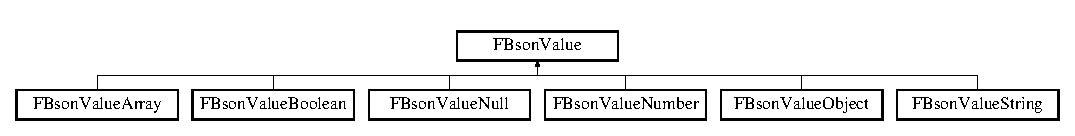
\includegraphics[height=1.382716cm]{class_f_bson_value}
\end{center}
\end{figure}
\subsection*{Public Member Functions}
\begin{DoxyCompactItemize}
\item 
double \mbox{\hyperlink{class_f_bson_value_ad23915f0921fb59d158a6ebf5ddfe5f9}{As\+Number}} () const
\item 
F\+String \mbox{\hyperlink{class_f_bson_value_aee42d2615ae788bd7374752b1c3a097d}{As\+String}} () const
\item 
bool \mbox{\hyperlink{class_f_bson_value_a0ec04eea92e4162d6887054ee8e3ab35}{As\+Bool}} () const
\item 
const T\+Array$<$ T\+Shared\+Ptr$<$ \mbox{\hyperlink{class_f_bson_value}{F\+Bson\+Value}} $>$ $>$ \& \mbox{\hyperlink{class_f_bson_value_a5a4a7cd0de121f66fd5ce0fbc78e86ed}{As\+Array}} () const
\item 
virtual const T\+Shared\+Ptr$<$ \mbox{\hyperlink{class_f_bson_object}{F\+Bson\+Object}} $>$ \& \mbox{\hyperlink{class_f_bson_value_a183af604be243a610b576dd7de32d334}{As\+Object}} () const
\item 
virtual bool \mbox{\hyperlink{class_f_bson_value_a519904f85122172ad9ca2f6b0b144f26}{Try\+Get\+Number}} (double \&Out\+Double) const
\item 
bool \mbox{\hyperlink{class_f_bson_value_a74a23bce29e9f699d0fde83663c4b3a8}{Try\+Get\+Number}} (int32 \&Out\+Number) const
\item 
bool \mbox{\hyperlink{class_f_bson_value_a5e61aa31b7c06178502e367957908e8c}{Try\+Get\+Number}} (uint32 \&Out\+Number) const
\item 
bool \mbox{\hyperlink{class_f_bson_value_a1e929bd6f5834d9a20658299605183f4}{Try\+Get\+Number}} (int64 \&Out\+Number) const
\item 
virtual bool \mbox{\hyperlink{class_f_bson_value_aa52379f3d911ed0d5c8ded6e83ceecc0}{Try\+Get\+String}} (F\+String \&Out\+String) const
\item 
virtual bool \mbox{\hyperlink{class_f_bson_value_a1c7d6b561d3cc8a7db99b850740c642e}{Try\+Get\+Bool}} (bool \&Out\+Bool) const
\item 
virtual bool \mbox{\hyperlink{class_f_bson_value_a80102a8570ea5468895c82f1bc480151}{Try\+Get\+Array}} (const T\+Array$<$ T\+Shared\+Ptr$<$ \mbox{\hyperlink{class_f_bson_value}{F\+Bson\+Value}} $>$$>$ $\ast$\&Out\+Array) const
\item 
virtual bool \mbox{\hyperlink{class_f_bson_value_a8f80bf7d02f1ac317a95fcc99776577b}{Try\+Get\+Object}} (const T\+Shared\+Ptr$<$ \mbox{\hyperlink{class_f_bson_object}{F\+Bson\+Object}} $>$ $\ast$\&Object) const
\item 
bool \mbox{\hyperlink{class_f_bson_value_a7f0281058bede8cfa8c7d8b4504d1995}{Is\+Null}} () const
\item 
void \mbox{\hyperlink{class_f_bson_value_a2776e2dccc09e36f42f5bc7f0412f79c}{As\+Argument\+Type}} (double \&Value)
\item 
\mbox{\Hypertarget{class_f_bson_value_a7516d8a132320bb62b149f4d8c98a66f}\label{class_f_bson_value_a7516d8a132320bb62b149f4d8c98a66f}} 
void {\bfseries As\+Argument\+Type} (F\+String \&Value)
\item 
\mbox{\Hypertarget{class_f_bson_value_a5296396a050c57e033ea348548d5fefc}\label{class_f_bson_value_a5296396a050c57e033ea348548d5fefc}} 
void {\bfseries As\+Argument\+Type} (bool \&Value)
\item 
\mbox{\Hypertarget{class_f_bson_value_aae3f6a5a9fb9b17c68a958aa82e457c1}\label{class_f_bson_value_aae3f6a5a9fb9b17c68a958aa82e457c1}} 
void {\bfseries As\+Argument\+Type} (T\+Array$<$ T\+Shared\+Ptr$<$ \mbox{\hyperlink{class_f_bson_value}{F\+Bson\+Value}} $>$$>$ \&Value)
\item 
\mbox{\Hypertarget{class_f_bson_value_aa0e81fc092785a8becd2228e281fd314}\label{class_f_bson_value_aa0e81fc092785a8becd2228e281fd314}} 
void {\bfseries As\+Argument\+Type} (T\+Shared\+Ptr$<$ \mbox{\hyperlink{class_f_bson_object}{F\+Bson\+Object}} $>$ \&Value)
\item 
bool \mbox{\hyperlink{class_f_bson_value_a245c10ded56b07a03099b71556d29073}{operator==}} (const \mbox{\hyperlink{class_f_bson_value}{F\+Bson\+Value}} \&Rhs) const
\end{DoxyCompactItemize}
\subsection*{Static Public Member Functions}
\begin{DoxyCompactItemize}
\item 
static bool \mbox{\hyperlink{class_f_bson_value_a979a25eef93a5f0398ecc372518a5c43}{Compare\+Equal}} (const \mbox{\hyperlink{class_f_bson_value}{F\+Bson\+Value}} \&Lhs, const \mbox{\hyperlink{class_f_bson_value}{F\+Bson\+Value}} \&Rhs)
\end{DoxyCompactItemize}
\subsection*{Public Attributes}
\begin{DoxyCompactItemize}
\item 
\mbox{\Hypertarget{class_f_bson_value_a36e564cf83ab781b52ea8d8e3e0be9b7}\label{class_f_bson_value_a36e564cf83ab781b52ea8d8e3e0be9b7}} 
E\+Bson {\bfseries Type}
\end{DoxyCompactItemize}
\subsection*{Protected Member Functions}
\begin{DoxyCompactItemize}
\item 
\mbox{\Hypertarget{class_f_bson_value_a6d3d6215d2ffd55c1445849b70dad5b5}\label{class_f_bson_value_a6d3d6215d2ffd55c1445849b70dad5b5}} 
virtual F\+String {\bfseries Get\+Type} () const =0
\item 
\mbox{\Hypertarget{class_f_bson_value_aa2f02c007e7ce6b465f328ded94cc66b}\label{class_f_bson_value_aa2f02c007e7ce6b465f328ded94cc66b}} 
void {\bfseries Error\+Message} (const F\+String \&In\+Type) const
\end{DoxyCompactItemize}
\subsection*{Static Protected Attributes}
\begin{DoxyCompactItemize}
\item 
\mbox{\Hypertarget{class_f_bson_value_a2b096906cada9314e9d4e42d723d2e8d}\label{class_f_bson_value_a2b096906cada9314e9d4e42d723d2e8d}} 
static const T\+Array$<$ T\+Shared\+Ptr$<$ \mbox{\hyperlink{class_f_bson_value}{F\+Bson\+Value}} $>$ $>$ {\bfseries E\+M\+P\+T\+Y\+\_\+\+A\+R\+R\+AY}
\item 
\mbox{\Hypertarget{class_f_bson_value_ac8abc326f63430015e2392e0abb6fd62}\label{class_f_bson_value_ac8abc326f63430015e2392e0abb6fd62}} 
static const T\+Shared\+Ptr$<$ \mbox{\hyperlink{class_f_bson_object}{F\+Bson\+Object}} $>$ {\bfseries E\+M\+P\+T\+Y\+\_\+\+O\+B\+J\+E\+CT}
\end{DoxyCompactItemize}


\subsection{Member Function Documentation}
\mbox{\Hypertarget{class_f_bson_value_a2776e2dccc09e36f42f5bc7f0412f79c}\label{class_f_bson_value_a2776e2dccc09e36f42f5bc7f0412f79c}} 
\index{F\+Bson\+Value@{F\+Bson\+Value}!As\+Argument\+Type@{As\+Argument\+Type}}
\index{As\+Argument\+Type@{As\+Argument\+Type}!F\+Bson\+Value@{F\+Bson\+Value}}
\subsubsection{\texorpdfstring{As\+Argument\+Type()}{AsArgumentType()}}
{\footnotesize\ttfamily void F\+Bson\+Value\+::\+As\+Argument\+Type (\begin{DoxyParamCaption}\item[{double \&}]{Value }\end{DoxyParamCaption})\hspace{0.3cm}{\ttfamily [inline]}}

Get a field of the same type as the argument. Mind that this uses the As\+Type functions which will return specified values if conversion isn\textquotesingle{}t possible.


\begin{DoxyParams}{Parameters}
{\em Value} & a reference of the desired type to put the converted value into. \\
\hline
\end{DoxyParams}
\mbox{\Hypertarget{class_f_bson_value_a5a4a7cd0de121f66fd5ce0fbc78e86ed}\label{class_f_bson_value_a5a4a7cd0de121f66fd5ce0fbc78e86ed}} 
\index{F\+Bson\+Value@{F\+Bson\+Value}!As\+Array@{As\+Array}}
\index{As\+Array@{As\+Array}!F\+Bson\+Value@{F\+Bson\+Value}}
\subsubsection{\texorpdfstring{As\+Array()}{AsArray()}}
{\footnotesize\ttfamily const T\+Array$<$T\+Shared\+Ptr$<$\mbox{\hyperlink{class_f_bson_value}{F\+Bson\+Value}}$>$ $>$\& F\+Bson\+Value\+::\+As\+Array (\begin{DoxyParamCaption}{ }\end{DoxyParamCaption}) const}

Returns this value as a T\+Array, logging an error and returning an empty T\+Array if not possible.

\begin{DoxyReturn}{Returns}
this value as a T\+Array or an empty T\+Array if it can\textquotesingle{}t be converted. 
\end{DoxyReturn}
\mbox{\Hypertarget{class_f_bson_value_a0ec04eea92e4162d6887054ee8e3ab35}\label{class_f_bson_value_a0ec04eea92e4162d6887054ee8e3ab35}} 
\index{F\+Bson\+Value@{F\+Bson\+Value}!As\+Bool@{As\+Bool}}
\index{As\+Bool@{As\+Bool}!F\+Bson\+Value@{F\+Bson\+Value}}
\subsubsection{\texorpdfstring{As\+Bool()}{AsBool()}}
{\footnotesize\ttfamily bool F\+Bson\+Value\+::\+As\+Bool (\begin{DoxyParamCaption}{ }\end{DoxyParamCaption}) const}

Returns this value as a boolean, logging an error and returning false if not possible.

\begin{DoxyReturn}{Returns}
this value as a boolean or false if it can\textquotesingle{}t be converted. 
\end{DoxyReturn}
\mbox{\Hypertarget{class_f_bson_value_ad23915f0921fb59d158a6ebf5ddfe5f9}\label{class_f_bson_value_ad23915f0921fb59d158a6ebf5ddfe5f9}} 
\index{F\+Bson\+Value@{F\+Bson\+Value}!As\+Number@{As\+Number}}
\index{As\+Number@{As\+Number}!F\+Bson\+Value@{F\+Bson\+Value}}
\subsubsection{\texorpdfstring{As\+Number()}{AsNumber()}}
{\footnotesize\ttfamily double F\+Bson\+Value\+::\+As\+Number (\begin{DoxyParamCaption}{ }\end{DoxyParamCaption}) const}

Returns this value as a double, logging an error and returning zero if not possible.

\begin{DoxyReturn}{Returns}
this value as a double or zero if it cant be converted. 
\end{DoxyReturn}
\mbox{\Hypertarget{class_f_bson_value_a183af604be243a610b576dd7de32d334}\label{class_f_bson_value_a183af604be243a610b576dd7de32d334}} 
\index{F\+Bson\+Value@{F\+Bson\+Value}!As\+Object@{As\+Object}}
\index{As\+Object@{As\+Object}!F\+Bson\+Value@{F\+Bson\+Value}}
\subsubsection{\texorpdfstring{As\+Object()}{AsObject()}}
{\footnotesize\ttfamily virtual const T\+Shared\+Ptr$<$\mbox{\hyperlink{class_f_bson_object}{F\+Bson\+Object}}$>$\& F\+Bson\+Value\+::\+As\+Object (\begin{DoxyParamCaption}{ }\end{DoxyParamCaption}) const\hspace{0.3cm}{\ttfamily [virtual]}}

Returns this value as an \mbox{\hyperlink{class_f_bson_object}{F\+Bson\+Object}}, throwing an error if this is not possible.

\begin{DoxyReturn}{Returns}
this value as an \mbox{\hyperlink{class_f_bson_object}{F\+Bson\+Object}}. 
\end{DoxyReturn}
\mbox{\Hypertarget{class_f_bson_value_aee42d2615ae788bd7374752b1c3a097d}\label{class_f_bson_value_aee42d2615ae788bd7374752b1c3a097d}} 
\index{F\+Bson\+Value@{F\+Bson\+Value}!As\+String@{As\+String}}
\index{As\+String@{As\+String}!F\+Bson\+Value@{F\+Bson\+Value}}
\subsubsection{\texorpdfstring{As\+String()}{AsString()}}
{\footnotesize\ttfamily F\+String F\+Bson\+Value\+::\+As\+String (\begin{DoxyParamCaption}{ }\end{DoxyParamCaption}) const}

Returns this value as a string, logging an error and returning an empty string if not possible.

\begin{DoxyReturn}{Returns}
this value as a string or an empty string if it can\textquotesingle{}t be converted. 
\end{DoxyReturn}
\mbox{\Hypertarget{class_f_bson_value_a979a25eef93a5f0398ecc372518a5c43}\label{class_f_bson_value_a979a25eef93a5f0398ecc372518a5c43}} 
\index{F\+Bson\+Value@{F\+Bson\+Value}!Compare\+Equal@{Compare\+Equal}}
\index{Compare\+Equal@{Compare\+Equal}!F\+Bson\+Value@{F\+Bson\+Value}}
\subsubsection{\texorpdfstring{Compare\+Equal()}{CompareEqual()}}
{\footnotesize\ttfamily static bool F\+Bson\+Value\+::\+Compare\+Equal (\begin{DoxyParamCaption}\item[{const \mbox{\hyperlink{class_f_bson_value}{F\+Bson\+Value}} \&}]{Lhs,  }\item[{const \mbox{\hyperlink{class_f_bson_value}{F\+Bson\+Value}} \&}]{Rhs }\end{DoxyParamCaption})\hspace{0.3cm}{\ttfamily [static]}}

Checks whether to F\+Bson\+Values are equal.


\begin{DoxyParams}{Parameters}
{\em Lhs} & first value to compare. \\
\hline
{\em Rhs} & second value to compare. \\
\hline
\end{DoxyParams}
\mbox{\Hypertarget{class_f_bson_value_a7f0281058bede8cfa8c7d8b4504d1995}\label{class_f_bson_value_a7f0281058bede8cfa8c7d8b4504d1995}} 
\index{F\+Bson\+Value@{F\+Bson\+Value}!Is\+Null@{Is\+Null}}
\index{Is\+Null@{Is\+Null}!F\+Bson\+Value@{F\+Bson\+Value}}
\subsubsection{\texorpdfstring{Is\+Null()}{IsNull()}}
{\footnotesize\ttfamily bool F\+Bson\+Value\+::\+Is\+Null (\begin{DoxyParamCaption}{ }\end{DoxyParamCaption}) const\hspace{0.3cm}{\ttfamily [inline]}}

\begin{DoxyReturn}{Returns}
true if this value is \textquotesingle{}null\textquotesingle{}. 
\end{DoxyReturn}
\mbox{\Hypertarget{class_f_bson_value_a245c10ded56b07a03099b71556d29073}\label{class_f_bson_value_a245c10ded56b07a03099b71556d29073}} 
\index{F\+Bson\+Value@{F\+Bson\+Value}!operator==@{operator==}}
\index{operator==@{operator==}!F\+Bson\+Value@{F\+Bson\+Value}}
\subsubsection{\texorpdfstring{operator==()}{operator==()}}
{\footnotesize\ttfamily bool F\+Bson\+Value\+::operator== (\begin{DoxyParamCaption}\item[{const \mbox{\hyperlink{class_f_bson_value}{F\+Bson\+Value}} \&}]{Rhs }\end{DoxyParamCaption}) const\hspace{0.3cm}{\ttfamily [inline]}}

Overloaded == operator that uses the \mbox{\hyperlink{class_f_bson_value_a979a25eef93a5f0398ecc372518a5c43}{Compare\+Equal()}} method for two F\+Bson\+Values. \mbox{\Hypertarget{class_f_bson_value_a80102a8570ea5468895c82f1bc480151}\label{class_f_bson_value_a80102a8570ea5468895c82f1bc480151}} 
\index{F\+Bson\+Value@{F\+Bson\+Value}!Try\+Get\+Array@{Try\+Get\+Array}}
\index{Try\+Get\+Array@{Try\+Get\+Array}!F\+Bson\+Value@{F\+Bson\+Value}}
\subsubsection{\texorpdfstring{Try\+Get\+Array()}{TryGetArray()}}
{\footnotesize\ttfamily virtual bool F\+Bson\+Value\+::\+Try\+Get\+Array (\begin{DoxyParamCaption}\item[{const T\+Array$<$ T\+Shared\+Ptr$<$ \mbox{\hyperlink{class_f_bson_value}{F\+Bson\+Value}} $>$$>$ $\ast$\&}]{Out\+Array }\end{DoxyParamCaption}) const\hspace{0.3cm}{\ttfamily [inline]}, {\ttfamily [virtual]}}

Tries to convert this value to a T\+Array of T\+Shared\+Ptr$<$\+F\+Bson\+Value$>$, returning false if not possible.


\begin{DoxyParams}{Parameters}
{\em Out\+Array} & a reference to write the converted T\+Array into. \\
\hline
\end{DoxyParams}
\begin{DoxyReturn}{Returns}
false if value can\textquotesingle{}t be converted, true otherwise. 
\end{DoxyReturn}


Reimplemented in \mbox{\hyperlink{class_f_bson_value_array_a32f100ae460cd26a870fc04d85ffe2c5}{F\+Bson\+Value\+Array}}.

\mbox{\Hypertarget{class_f_bson_value_a1c7d6b561d3cc8a7db99b850740c642e}\label{class_f_bson_value_a1c7d6b561d3cc8a7db99b850740c642e}} 
\index{F\+Bson\+Value@{F\+Bson\+Value}!Try\+Get\+Bool@{Try\+Get\+Bool}}
\index{Try\+Get\+Bool@{Try\+Get\+Bool}!F\+Bson\+Value@{F\+Bson\+Value}}
\subsubsection{\texorpdfstring{Try\+Get\+Bool()}{TryGetBool()}}
{\footnotesize\ttfamily virtual bool F\+Bson\+Value\+::\+Try\+Get\+Bool (\begin{DoxyParamCaption}\item[{bool \&}]{Out\+Bool }\end{DoxyParamCaption}) const\hspace{0.3cm}{\ttfamily [inline]}, {\ttfamily [virtual]}}

Tries to convert this value to an boolean, returning false if not possible.


\begin{DoxyParams}{Parameters}
{\em Out\+Bool} & a reference to write the converted boolean into. \\
\hline
\end{DoxyParams}
\begin{DoxyReturn}{Returns}
false if value can\textquotesingle{}t be converted, true otherwise. 
\end{DoxyReturn}


Reimplemented in \mbox{\hyperlink{class_f_bson_value_boolean_a1999907437ed5dc5142f46919683c478}{F\+Bson\+Value\+Boolean}}, \mbox{\hyperlink{class_f_bson_value_number_af85e6c473afae0cb5340499ab013cf4f}{F\+Bson\+Value\+Number}}, and \mbox{\hyperlink{class_f_bson_value_string_a81c2e67998032708c613773746c962bd}{F\+Bson\+Value\+String}}.

\mbox{\Hypertarget{class_f_bson_value_a519904f85122172ad9ca2f6b0b144f26}\label{class_f_bson_value_a519904f85122172ad9ca2f6b0b144f26}} 
\index{F\+Bson\+Value@{F\+Bson\+Value}!Try\+Get\+Number@{Try\+Get\+Number}}
\index{Try\+Get\+Number@{Try\+Get\+Number}!F\+Bson\+Value@{F\+Bson\+Value}}
\subsubsection{\texorpdfstring{Try\+Get\+Number()}{TryGetNumber()}\hspace{0.1cm}{\footnotesize\ttfamily [1/4]}}
{\footnotesize\ttfamily virtual bool F\+Bson\+Value\+::\+Try\+Get\+Number (\begin{DoxyParamCaption}\item[{double \&}]{Out\+Double }\end{DoxyParamCaption}) const\hspace{0.3cm}{\ttfamily [inline]}, {\ttfamily [virtual]}}

Tries to convert this value to a double, returning false if not possible.


\begin{DoxyParams}{Parameters}
{\em Out\+Double} & a reference to write the converted number into. \\
\hline
\end{DoxyParams}
\begin{DoxyReturn}{Returns}
false if value can\textquotesingle{}t be converted, true otherwise. 
\end{DoxyReturn}


Reimplemented in \mbox{\hyperlink{class_f_bson_value_boolean_a7c46553a8c6caaec96ce0821977ee1e7}{F\+Bson\+Value\+Boolean}}, \mbox{\hyperlink{class_f_bson_value_number_a6e5788ee9637c76e073c6336f1b3d263}{F\+Bson\+Value\+Number}}, and \mbox{\hyperlink{class_f_bson_value_string_a7346681867daa27d7fa4a4e690ba55aa}{F\+Bson\+Value\+String}}.

\mbox{\Hypertarget{class_f_bson_value_a74a23bce29e9f699d0fde83663c4b3a8}\label{class_f_bson_value_a74a23bce29e9f699d0fde83663c4b3a8}} 
\index{F\+Bson\+Value@{F\+Bson\+Value}!Try\+Get\+Number@{Try\+Get\+Number}}
\index{Try\+Get\+Number@{Try\+Get\+Number}!F\+Bson\+Value@{F\+Bson\+Value}}
\subsubsection{\texorpdfstring{Try\+Get\+Number()}{TryGetNumber()}\hspace{0.1cm}{\footnotesize\ttfamily [2/4]}}
{\footnotesize\ttfamily bool F\+Bson\+Value\+::\+Try\+Get\+Number (\begin{DoxyParamCaption}\item[{int32 \&}]{Out\+Number }\end{DoxyParamCaption}) const}

Tries to convert this value to an int32, returning false if not possible.


\begin{DoxyParams}{Parameters}
{\em Out\+Number} & a reference to write the converted number into. \\
\hline
\end{DoxyParams}
\begin{DoxyReturn}{Returns}
false if value can\textquotesingle{}t be converted, true otherwise. 
\end{DoxyReturn}
\mbox{\Hypertarget{class_f_bson_value_a5e61aa31b7c06178502e367957908e8c}\label{class_f_bson_value_a5e61aa31b7c06178502e367957908e8c}} 
\index{F\+Bson\+Value@{F\+Bson\+Value}!Try\+Get\+Number@{Try\+Get\+Number}}
\index{Try\+Get\+Number@{Try\+Get\+Number}!F\+Bson\+Value@{F\+Bson\+Value}}
\subsubsection{\texorpdfstring{Try\+Get\+Number()}{TryGetNumber()}\hspace{0.1cm}{\footnotesize\ttfamily [3/4]}}
{\footnotesize\ttfamily bool F\+Bson\+Value\+::\+Try\+Get\+Number (\begin{DoxyParamCaption}\item[{uint32 \&}]{Out\+Number }\end{DoxyParamCaption}) const}

Tries to convert this value to a uint32, returning false if not possible.


\begin{DoxyParams}{Parameters}
{\em Out\+Number} & a reference to write the converted number into. \\
\hline
\end{DoxyParams}
\begin{DoxyReturn}{Returns}
false if value can\textquotesingle{}t be converted, true otherwise. 
\end{DoxyReturn}
\mbox{\Hypertarget{class_f_bson_value_a1e929bd6f5834d9a20658299605183f4}\label{class_f_bson_value_a1e929bd6f5834d9a20658299605183f4}} 
\index{F\+Bson\+Value@{F\+Bson\+Value}!Try\+Get\+Number@{Try\+Get\+Number}}
\index{Try\+Get\+Number@{Try\+Get\+Number}!F\+Bson\+Value@{F\+Bson\+Value}}
\subsubsection{\texorpdfstring{Try\+Get\+Number()}{TryGetNumber()}\hspace{0.1cm}{\footnotesize\ttfamily [4/4]}}
{\footnotesize\ttfamily bool F\+Bson\+Value\+::\+Try\+Get\+Number (\begin{DoxyParamCaption}\item[{int64 \&}]{Out\+Number }\end{DoxyParamCaption}) const}

Tries to convert this value to an int64, returning false if not possible.


\begin{DoxyParams}{Parameters}
{\em Out\+Number} & a reference to write the converted number into. \\
\hline
\end{DoxyParams}
\begin{DoxyReturn}{Returns}
false if value can\textquotesingle{}t be converted, true otherwise. 
\end{DoxyReturn}
\mbox{\Hypertarget{class_f_bson_value_a8f80bf7d02f1ac317a95fcc99776577b}\label{class_f_bson_value_a8f80bf7d02f1ac317a95fcc99776577b}} 
\index{F\+Bson\+Value@{F\+Bson\+Value}!Try\+Get\+Object@{Try\+Get\+Object}}
\index{Try\+Get\+Object@{Try\+Get\+Object}!F\+Bson\+Value@{F\+Bson\+Value}}
\subsubsection{\texorpdfstring{Try\+Get\+Object()}{TryGetObject()}}
{\footnotesize\ttfamily virtual bool F\+Bson\+Value\+::\+Try\+Get\+Object (\begin{DoxyParamCaption}\item[{const T\+Shared\+Ptr$<$ \mbox{\hyperlink{class_f_bson_object}{F\+Bson\+Object}} $>$ $\ast$\&}]{Object }\end{DoxyParamCaption}) const\hspace{0.3cm}{\ttfamily [inline]}, {\ttfamily [virtual]}}

Tries to convert this value to an \mbox{\hyperlink{class_f_bson_object}{F\+Bson\+Object}}, returning false if not possible.


\begin{DoxyParams}{Parameters}
{\em Object} & a pointer to a reference to write the converted Object into. \\
\hline
\end{DoxyParams}
\begin{DoxyReturn}{Returns}
false if value can\textquotesingle{}t be converted, true otherwise. 
\end{DoxyReturn}


Reimplemented in \mbox{\hyperlink{class_f_bson_value_object_adf5ee6fb14cdfea399c4c25a4778a414}{F\+Bson\+Value\+Object}}.

\mbox{\Hypertarget{class_f_bson_value_aa52379f3d911ed0d5c8ded6e83ceecc0}\label{class_f_bson_value_aa52379f3d911ed0d5c8ded6e83ceecc0}} 
\index{F\+Bson\+Value@{F\+Bson\+Value}!Try\+Get\+String@{Try\+Get\+String}}
\index{Try\+Get\+String@{Try\+Get\+String}!F\+Bson\+Value@{F\+Bson\+Value}}
\subsubsection{\texorpdfstring{Try\+Get\+String()}{TryGetString()}}
{\footnotesize\ttfamily virtual bool F\+Bson\+Value\+::\+Try\+Get\+String (\begin{DoxyParamCaption}\item[{F\+String \&}]{Out\+String }\end{DoxyParamCaption}) const\hspace{0.3cm}{\ttfamily [inline]}, {\ttfamily [virtual]}}

Tries to convert this value to an F\+String, returning false if not possible.


\begin{DoxyParams}{Parameters}
{\em Out\+String} & a reference to write the converted F\+String into. \\
\hline
\end{DoxyParams}
\begin{DoxyReturn}{Returns}
false if value can\textquotesingle{}t be converted, true otherwise. 
\end{DoxyReturn}


Reimplemented in \mbox{\hyperlink{class_f_bson_value_boolean_ace6ca5efe35c941d7b9d9f6a9df0ef02}{F\+Bson\+Value\+Boolean}}, \mbox{\hyperlink{class_f_bson_value_number_a7a8298e9a37d8d93f5b37319665e6735}{F\+Bson\+Value\+Number}}, and \mbox{\hyperlink{class_f_bson_value_string_a531bcc8511d8de17418fd7fe6d0d797f}{F\+Bson\+Value\+String}}.



The documentation for this class was generated from the following file\+:\begin{DoxyCompactItemize}
\item 
Bson\+Value.\+h\end{DoxyCompactItemize}

\hypertarget{class_f_bson_value_array}{}\section{F\+Bson\+Value\+Array Class Reference}
\label{class_f_bson_value_array}\index{F\+Bson\+Value\+Array@{F\+Bson\+Value\+Array}}


{\ttfamily \#include $<$Bson\+Value.\+h$>$}

Inheritance diagram for F\+Bson\+Value\+Array\+:\begin{figure}[H]
\begin{center}
\leavevmode
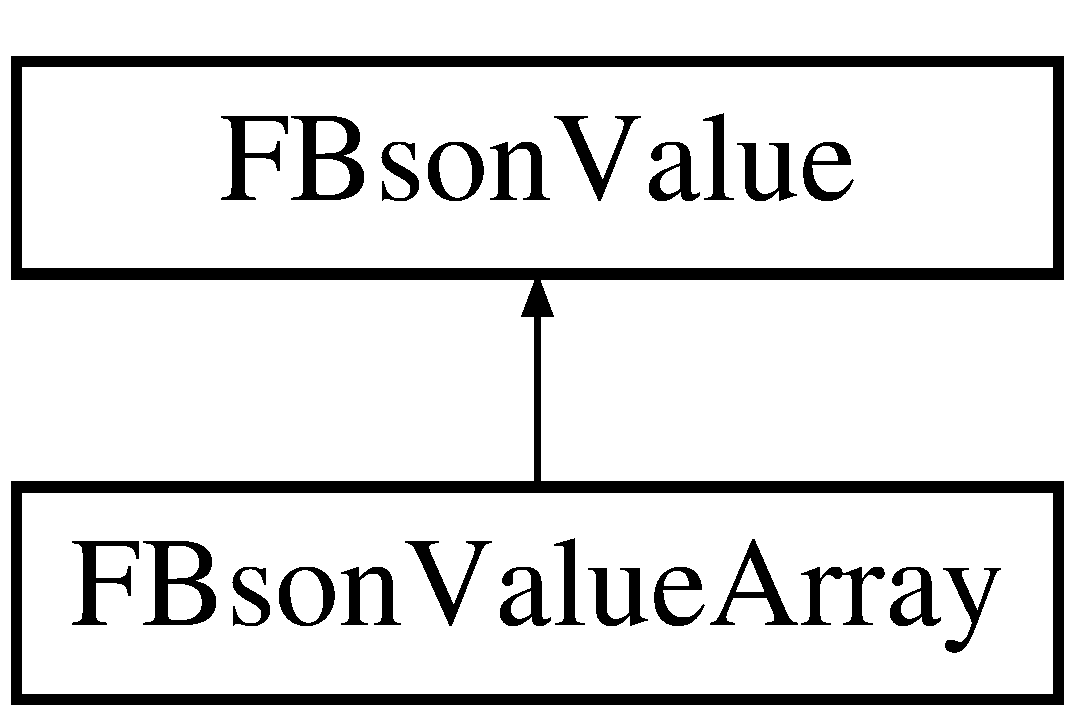
\includegraphics[height=2.000000cm]{class_f_bson_value_array}
\end{center}
\end{figure}
\subsection*{Public Member Functions}
\begin{DoxyCompactItemize}
\item 
\mbox{\Hypertarget{class_f_bson_value_array_a1101ddb368136fa040bd3340446e2e58}\label{class_f_bson_value_array_a1101ddb368136fa040bd3340446e2e58}} 
{\bfseries F\+Bson\+Value\+Array} (const T\+Array$<$ T\+Shared\+Ptr$<$ \mbox{\hyperlink{class_f_bson_value}{F\+Bson\+Value}} $>$$>$ \&In\+Array)
\item 
virtual bool \mbox{\hyperlink{class_f_bson_value_array_a32f100ae460cd26a870fc04d85ffe2c5}{Try\+Get\+Array}} (const T\+Array$<$ T\+Shared\+Ptr$<$ \mbox{\hyperlink{class_f_bson_value}{F\+Bson\+Value}} $>$$>$ $\ast$\&Out\+Array) const override
\end{DoxyCompactItemize}
\subsection*{Protected Member Functions}
\begin{DoxyCompactItemize}
\item 
\mbox{\Hypertarget{class_f_bson_value_array_a30a33b8e9f808aaa049df54819380175}\label{class_f_bson_value_array_a30a33b8e9f808aaa049df54819380175}} 
virtual F\+String {\bfseries Get\+Type} () const override
\end{DoxyCompactItemize}
\subsection*{Protected Attributes}
\begin{DoxyCompactItemize}
\item 
\mbox{\Hypertarget{class_f_bson_value_array_a677992b370839f3b2b1831698b986a00}\label{class_f_bson_value_array_a677992b370839f3b2b1831698b986a00}} 
T\+Array$<$ T\+Shared\+Ptr$<$ \mbox{\hyperlink{class_f_bson_value}{F\+Bson\+Value}} $>$ $>$ {\bfseries Value}
\end{DoxyCompactItemize}
\subsection*{Additional Inherited Members}


\subsection{Detailed Description}
A Json Array Value. 

\subsection{Member Function Documentation}
\mbox{\Hypertarget{class_f_bson_value_array_a32f100ae460cd26a870fc04d85ffe2c5}\label{class_f_bson_value_array_a32f100ae460cd26a870fc04d85ffe2c5}} 
\index{F\+Bson\+Value\+Array@{F\+Bson\+Value\+Array}!Try\+Get\+Array@{Try\+Get\+Array}}
\index{Try\+Get\+Array@{Try\+Get\+Array}!F\+Bson\+Value\+Array@{F\+Bson\+Value\+Array}}
\subsubsection{\texorpdfstring{Try\+Get\+Array()}{TryGetArray()}}
{\footnotesize\ttfamily virtual bool F\+Bson\+Value\+Array\+::\+Try\+Get\+Array (\begin{DoxyParamCaption}\item[{const T\+Array$<$ T\+Shared\+Ptr$<$ \mbox{\hyperlink{class_f_bson_value}{F\+Bson\+Value}} $>$$>$ $\ast$\&}]{Out\+Array }\end{DoxyParamCaption}) const\hspace{0.3cm}{\ttfamily [inline]}, {\ttfamily [override]}, {\ttfamily [virtual]}}

Tries to convert this value to a T\+Array of T\+Shared\+Ptr$<$\+F\+Bson\+Value$>$, returning false if not possible.


\begin{DoxyParams}{Parameters}
{\em Out\+Array} & a reference to write the converted T\+Array into. \\
\hline
\end{DoxyParams}
\begin{DoxyReturn}{Returns}
false if value can\textquotesingle{}t be converted, true otherwise. 
\end{DoxyReturn}


Reimplemented from \mbox{\hyperlink{class_f_bson_value_a80102a8570ea5468895c82f1bc480151}{F\+Bson\+Value}}.



The documentation for this class was generated from the following file\+:\begin{DoxyCompactItemize}
\item 
Bson\+Value.\+h\end{DoxyCompactItemize}

\hypertarget{class_f_bson_value_boolean}{}\section{F\+Bson\+Value\+Boolean Class Reference}
\label{class_f_bson_value_boolean}\index{F\+Bson\+Value\+Boolean@{F\+Bson\+Value\+Boolean}}


{\ttfamily \#include $<$Bson\+Value.\+h$>$}

Inheritance diagram for F\+Bson\+Value\+Boolean\+:\begin{figure}[H]
\begin{center}
\leavevmode
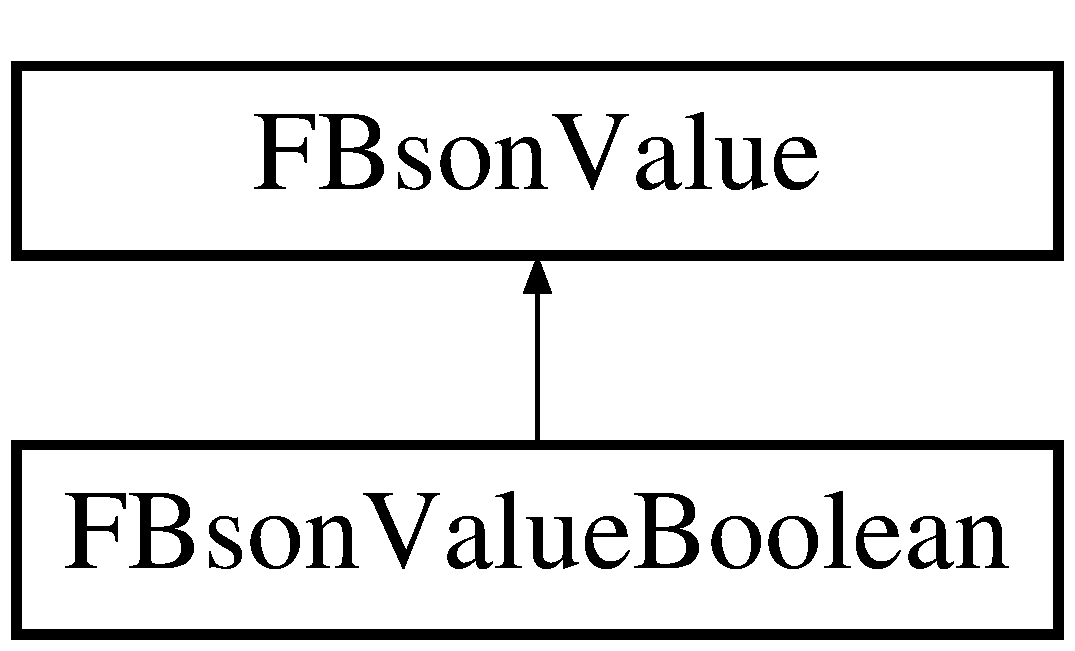
\includegraphics[height=2.000000cm]{class_f_bson_value_boolean}
\end{center}
\end{figure}
\subsection*{Public Member Functions}
\begin{DoxyCompactItemize}
\item 
\mbox{\Hypertarget{class_f_bson_value_boolean_a35ec849ce478e3e30520d152c582d745}\label{class_f_bson_value_boolean_a35ec849ce478e3e30520d152c582d745}} 
{\bfseries F\+Bson\+Value\+Boolean} (bool In\+Bool)
\item 
virtual bool \mbox{\hyperlink{class_f_bson_value_boolean_a7c46553a8c6caaec96ce0821977ee1e7}{Try\+Get\+Number}} (double \&Out\+Number) const override
\item 
virtual bool \mbox{\hyperlink{class_f_bson_value_boolean_a1999907437ed5dc5142f46919683c478}{Try\+Get\+Bool}} (bool \&Out\+Bool) const override
\item 
virtual bool \mbox{\hyperlink{class_f_bson_value_boolean_ace6ca5efe35c941d7b9d9f6a9df0ef02}{Try\+Get\+String}} (F\+String \&Out\+String) const override
\end{DoxyCompactItemize}
\subsection*{Protected Member Functions}
\begin{DoxyCompactItemize}
\item 
\mbox{\Hypertarget{class_f_bson_value_boolean_aed853cf29de96c87ac5614a4ecd3b53b}\label{class_f_bson_value_boolean_aed853cf29de96c87ac5614a4ecd3b53b}} 
virtual F\+String {\bfseries Get\+Type} () const override
\end{DoxyCompactItemize}
\subsection*{Protected Attributes}
\begin{DoxyCompactItemize}
\item 
\mbox{\Hypertarget{class_f_bson_value_boolean_ad15c81e2806941eb37091102f3d81cea}\label{class_f_bson_value_boolean_ad15c81e2806941eb37091102f3d81cea}} 
bool {\bfseries Value}
\end{DoxyCompactItemize}
\subsection*{Additional Inherited Members}


\subsection{Detailed Description}
A Bson Boolean Value. 

\subsection{Member Function Documentation}
\mbox{\Hypertarget{class_f_bson_value_boolean_a1999907437ed5dc5142f46919683c478}\label{class_f_bson_value_boolean_a1999907437ed5dc5142f46919683c478}} 
\index{F\+Bson\+Value\+Boolean@{F\+Bson\+Value\+Boolean}!Try\+Get\+Bool@{Try\+Get\+Bool}}
\index{Try\+Get\+Bool@{Try\+Get\+Bool}!F\+Bson\+Value\+Boolean@{F\+Bson\+Value\+Boolean}}
\subsubsection{\texorpdfstring{Try\+Get\+Bool()}{TryGetBool()}}
{\footnotesize\ttfamily virtual bool F\+Bson\+Value\+Boolean\+::\+Try\+Get\+Bool (\begin{DoxyParamCaption}\item[{bool \&}]{Out\+Bool }\end{DoxyParamCaption}) const\hspace{0.3cm}{\ttfamily [inline]}, {\ttfamily [override]}, {\ttfamily [virtual]}}

Tries to convert this value to an boolean, returning false if not possible.


\begin{DoxyParams}{Parameters}
{\em Out\+Bool} & a reference to write the converted boolean into. \\
\hline
\end{DoxyParams}
\begin{DoxyReturn}{Returns}
false if value can\textquotesingle{}t be converted, true otherwise. 
\end{DoxyReturn}


Reimplemented from \mbox{\hyperlink{class_f_bson_value_a1c7d6b561d3cc8a7db99b850740c642e}{F\+Bson\+Value}}.

\mbox{\Hypertarget{class_f_bson_value_boolean_a7c46553a8c6caaec96ce0821977ee1e7}\label{class_f_bson_value_boolean_a7c46553a8c6caaec96ce0821977ee1e7}} 
\index{F\+Bson\+Value\+Boolean@{F\+Bson\+Value\+Boolean}!Try\+Get\+Number@{Try\+Get\+Number}}
\index{Try\+Get\+Number@{Try\+Get\+Number}!F\+Bson\+Value\+Boolean@{F\+Bson\+Value\+Boolean}}
\subsubsection{\texorpdfstring{Try\+Get\+Number()}{TryGetNumber()}}
{\footnotesize\ttfamily virtual bool F\+Bson\+Value\+Boolean\+::\+Try\+Get\+Number (\begin{DoxyParamCaption}\item[{double \&}]{Out\+Double }\end{DoxyParamCaption}) const\hspace{0.3cm}{\ttfamily [inline]}, {\ttfamily [override]}, {\ttfamily [virtual]}}

Tries to convert this value to a double, returning false if not possible.


\begin{DoxyParams}{Parameters}
{\em Out\+Double} & a reference to write the converted number into. \\
\hline
\end{DoxyParams}
\begin{DoxyReturn}{Returns}
false if value can\textquotesingle{}t be converted, true otherwise. 
\end{DoxyReturn}


Reimplemented from \mbox{\hyperlink{class_f_bson_value_a519904f85122172ad9ca2f6b0b144f26}{F\+Bson\+Value}}.

\mbox{\Hypertarget{class_f_bson_value_boolean_ace6ca5efe35c941d7b9d9f6a9df0ef02}\label{class_f_bson_value_boolean_ace6ca5efe35c941d7b9d9f6a9df0ef02}} 
\index{F\+Bson\+Value\+Boolean@{F\+Bson\+Value\+Boolean}!Try\+Get\+String@{Try\+Get\+String}}
\index{Try\+Get\+String@{Try\+Get\+String}!F\+Bson\+Value\+Boolean@{F\+Bson\+Value\+Boolean}}
\subsubsection{\texorpdfstring{Try\+Get\+String()}{TryGetString()}}
{\footnotesize\ttfamily virtual bool F\+Bson\+Value\+Boolean\+::\+Try\+Get\+String (\begin{DoxyParamCaption}\item[{F\+String \&}]{Out\+String }\end{DoxyParamCaption}) const\hspace{0.3cm}{\ttfamily [inline]}, {\ttfamily [override]}, {\ttfamily [virtual]}}

Tries to convert this value to an F\+String, returning false if not possible.


\begin{DoxyParams}{Parameters}
{\em Out\+String} & a reference to write the converted F\+String into. \\
\hline
\end{DoxyParams}
\begin{DoxyReturn}{Returns}
false if value can\textquotesingle{}t be converted, true otherwise. 
\end{DoxyReturn}


Reimplemented from \mbox{\hyperlink{class_f_bson_value_aa52379f3d911ed0d5c8ded6e83ceecc0}{F\+Bson\+Value}}.



The documentation for this class was generated from the following file\+:\begin{DoxyCompactItemize}
\item 
Bson\+Value.\+h\end{DoxyCompactItemize}

\hypertarget{class_f_bson_value_null}{}\section{F\+Bson\+Value\+Null Class Reference}
\label{class_f_bson_value_null}\index{F\+Bson\+Value\+Null@{F\+Bson\+Value\+Null}}


{\ttfamily \#include $<$Bson\+Value.\+h$>$}

Inheritance diagram for F\+Bson\+Value\+Null\+:\begin{figure}[H]
\begin{center}
\leavevmode
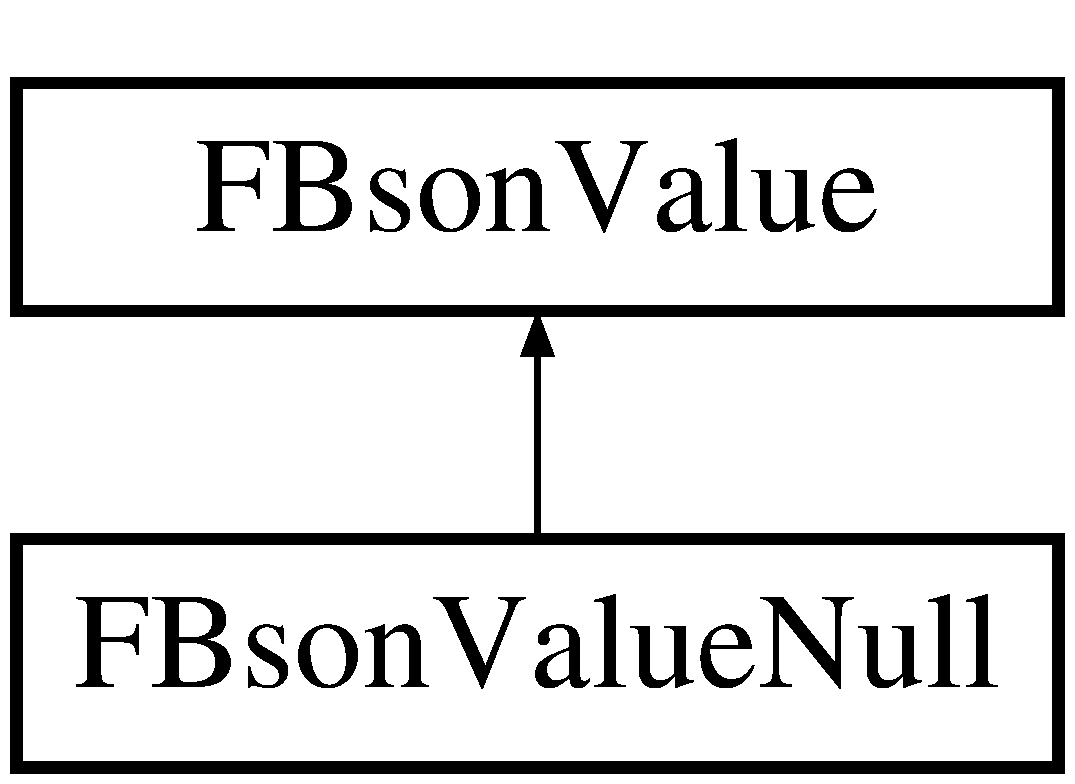
\includegraphics[height=2.000000cm]{class_f_bson_value_null}
\end{center}
\end{figure}
\subsection*{Protected Member Functions}
\begin{DoxyCompactItemize}
\item 
\mbox{\Hypertarget{class_f_bson_value_null_ab34e6a39108cc1f8fad4db16c453c3b6}\label{class_f_bson_value_null_ab34e6a39108cc1f8fad4db16c453c3b6}} 
virtual F\+String {\bfseries Get\+Type} () const override
\end{DoxyCompactItemize}
\subsection*{Additional Inherited Members}


\subsection{Detailed Description}
A Bson Null Value. 

The documentation for this class was generated from the following file\+:\begin{DoxyCompactItemize}
\item 
Bson\+Value.\+h\end{DoxyCompactItemize}

\hypertarget{class_f_bson_value_number}{}\section{F\+Bson\+Value\+Number Class Reference}
\label{class_f_bson_value_number}\index{F\+Bson\+Value\+Number@{F\+Bson\+Value\+Number}}


{\ttfamily \#include $<$Bson\+Value.\+h$>$}

Inheritance diagram for F\+Bson\+Value\+Number\+:\begin{figure}[H]
\begin{center}
\leavevmode
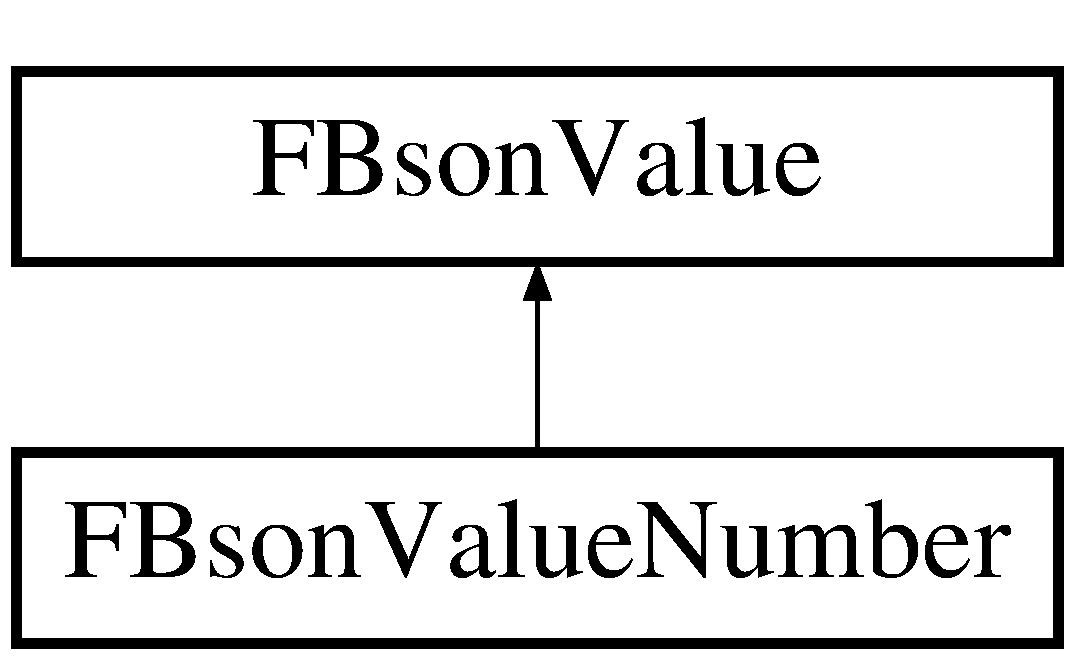
\includegraphics[height=2.000000cm]{class_f_bson_value_number}
\end{center}
\end{figure}
\subsection*{Public Member Functions}
\begin{DoxyCompactItemize}
\item 
\mbox{\Hypertarget{class_f_bson_value_number_a455bbd7ddd29d2dddacfa5d479bbd6c7}\label{class_f_bson_value_number_a455bbd7ddd29d2dddacfa5d479bbd6c7}} 
{\bfseries F\+Bson\+Value\+Number} (double In\+Number)
\item 
virtual bool \mbox{\hyperlink{class_f_bson_value_number_a6e5788ee9637c76e073c6336f1b3d263}{Try\+Get\+Number}} (double \&Out\+Number) const override
\item 
virtual bool \mbox{\hyperlink{class_f_bson_value_number_af85e6c473afae0cb5340499ab013cf4f}{Try\+Get\+Bool}} (bool \&Out\+Bool) const override
\item 
virtual bool \mbox{\hyperlink{class_f_bson_value_number_a7a8298e9a37d8d93f5b37319665e6735}{Try\+Get\+String}} (F\+String \&Out\+String) const override
\end{DoxyCompactItemize}
\subsection*{Protected Member Functions}
\begin{DoxyCompactItemize}
\item 
\mbox{\Hypertarget{class_f_bson_value_number_a4efd450f2e77f179f682e809ff8313e5}\label{class_f_bson_value_number_a4efd450f2e77f179f682e809ff8313e5}} 
virtual F\+String {\bfseries Get\+Type} () const override
\end{DoxyCompactItemize}
\subsection*{Protected Attributes}
\begin{DoxyCompactItemize}
\item 
\mbox{\Hypertarget{class_f_bson_value_number_a37e55c82055b7e09df5ff477013b5b5c}\label{class_f_bson_value_number_a37e55c82055b7e09df5ff477013b5b5c}} 
double {\bfseries Value}
\end{DoxyCompactItemize}
\subsection*{Additional Inherited Members}


\subsection{Detailed Description}
A Bson Number Value. 

\subsection{Member Function Documentation}
\mbox{\Hypertarget{class_f_bson_value_number_af85e6c473afae0cb5340499ab013cf4f}\label{class_f_bson_value_number_af85e6c473afae0cb5340499ab013cf4f}} 
\index{F\+Bson\+Value\+Number@{F\+Bson\+Value\+Number}!Try\+Get\+Bool@{Try\+Get\+Bool}}
\index{Try\+Get\+Bool@{Try\+Get\+Bool}!F\+Bson\+Value\+Number@{F\+Bson\+Value\+Number}}
\subsubsection{\texorpdfstring{Try\+Get\+Bool()}{TryGetBool()}}
{\footnotesize\ttfamily virtual bool F\+Bson\+Value\+Number\+::\+Try\+Get\+Bool (\begin{DoxyParamCaption}\item[{bool \&}]{Out\+Bool }\end{DoxyParamCaption}) const\hspace{0.3cm}{\ttfamily [inline]}, {\ttfamily [override]}, {\ttfamily [virtual]}}

Tries to convert this value to an boolean, returning false if not possible.


\begin{DoxyParams}{Parameters}
{\em Out\+Bool} & a reference to write the converted boolean into. \\
\hline
\end{DoxyParams}
\begin{DoxyReturn}{Returns}
false if value can\textquotesingle{}t be converted, true otherwise. 
\end{DoxyReturn}


Reimplemented from \mbox{\hyperlink{class_f_bson_value_a1c7d6b561d3cc8a7db99b850740c642e}{F\+Bson\+Value}}.

\mbox{\Hypertarget{class_f_bson_value_number_a6e5788ee9637c76e073c6336f1b3d263}\label{class_f_bson_value_number_a6e5788ee9637c76e073c6336f1b3d263}} 
\index{F\+Bson\+Value\+Number@{F\+Bson\+Value\+Number}!Try\+Get\+Number@{Try\+Get\+Number}}
\index{Try\+Get\+Number@{Try\+Get\+Number}!F\+Bson\+Value\+Number@{F\+Bson\+Value\+Number}}
\subsubsection{\texorpdfstring{Try\+Get\+Number()}{TryGetNumber()}}
{\footnotesize\ttfamily virtual bool F\+Bson\+Value\+Number\+::\+Try\+Get\+Number (\begin{DoxyParamCaption}\item[{double \&}]{Out\+Double }\end{DoxyParamCaption}) const\hspace{0.3cm}{\ttfamily [inline]}, {\ttfamily [override]}, {\ttfamily [virtual]}}

Tries to convert this value to a double, returning false if not possible.


\begin{DoxyParams}{Parameters}
{\em Out\+Double} & a reference to write the converted number into. \\
\hline
\end{DoxyParams}
\begin{DoxyReturn}{Returns}
false if value can\textquotesingle{}t be converted, true otherwise. 
\end{DoxyReturn}


Reimplemented from \mbox{\hyperlink{class_f_bson_value_a519904f85122172ad9ca2f6b0b144f26}{F\+Bson\+Value}}.

\mbox{\Hypertarget{class_f_bson_value_number_a7a8298e9a37d8d93f5b37319665e6735}\label{class_f_bson_value_number_a7a8298e9a37d8d93f5b37319665e6735}} 
\index{F\+Bson\+Value\+Number@{F\+Bson\+Value\+Number}!Try\+Get\+String@{Try\+Get\+String}}
\index{Try\+Get\+String@{Try\+Get\+String}!F\+Bson\+Value\+Number@{F\+Bson\+Value\+Number}}
\subsubsection{\texorpdfstring{Try\+Get\+String()}{TryGetString()}}
{\footnotesize\ttfamily virtual bool F\+Bson\+Value\+Number\+::\+Try\+Get\+String (\begin{DoxyParamCaption}\item[{F\+String \&}]{Out\+String }\end{DoxyParamCaption}) const\hspace{0.3cm}{\ttfamily [inline]}, {\ttfamily [override]}, {\ttfamily [virtual]}}

Tries to convert this value to an F\+String, returning false if not possible.


\begin{DoxyParams}{Parameters}
{\em Out\+String} & a reference to write the converted F\+String into. \\
\hline
\end{DoxyParams}
\begin{DoxyReturn}{Returns}
false if value can\textquotesingle{}t be converted, true otherwise. 
\end{DoxyReturn}


Reimplemented from \mbox{\hyperlink{class_f_bson_value_aa52379f3d911ed0d5c8ded6e83ceecc0}{F\+Bson\+Value}}.



The documentation for this class was generated from the following file\+:\begin{DoxyCompactItemize}
\item 
Bson\+Value.\+h\end{DoxyCompactItemize}

\hypertarget{class_f_bson_value_object}{}\section{F\+Bson\+Value\+Object Class Reference}
\label{class_f_bson_value_object}\index{F\+Bson\+Value\+Object@{F\+Bson\+Value\+Object}}


{\ttfamily \#include $<$Bson\+Value.\+h$>$}

Inheritance diagram for F\+Bson\+Value\+Object\+:\begin{figure}[H]
\begin{center}
\leavevmode
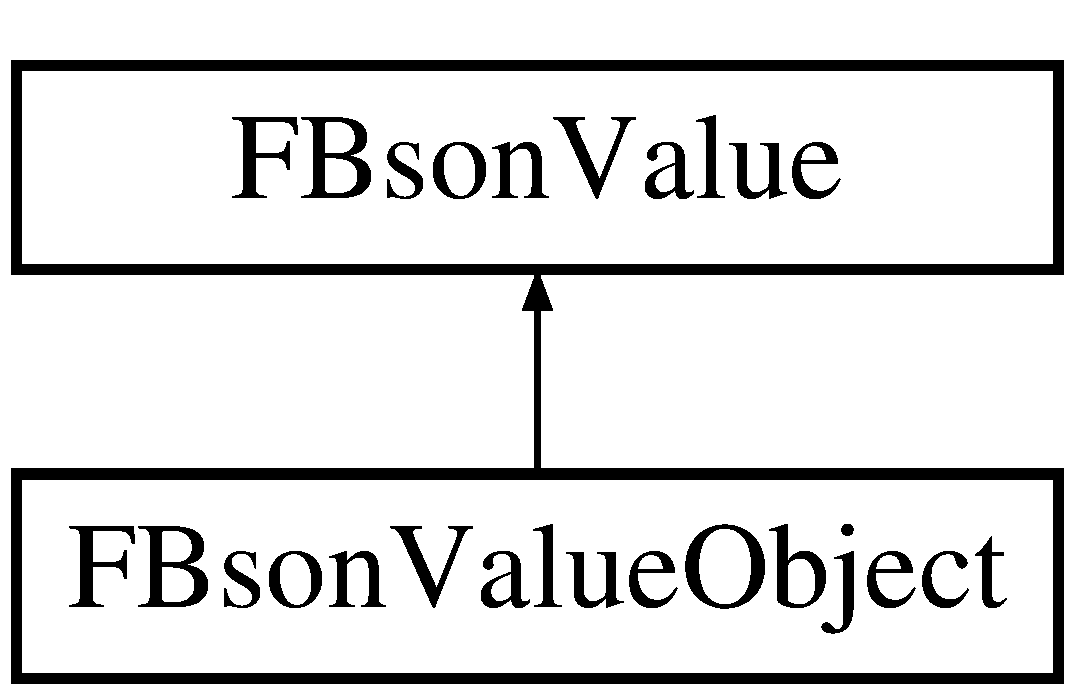
\includegraphics[height=2.000000cm]{class_f_bson_value_object}
\end{center}
\end{figure}
\subsection*{Public Member Functions}
\begin{DoxyCompactItemize}
\item 
\mbox{\Hypertarget{class_f_bson_value_object_a910522eb48a9c7eb710b519b1b4ff222}\label{class_f_bson_value_object_a910522eb48a9c7eb710b519b1b4ff222}} 
{\bfseries F\+Bson\+Value\+Object} (T\+Shared\+Ptr$<$ \mbox{\hyperlink{class_f_bson_object}{F\+Bson\+Object}} $>$ In\+Object)
\item 
virtual bool \mbox{\hyperlink{class_f_bson_value_object_adf5ee6fb14cdfea399c4c25a4778a414}{Try\+Get\+Object}} (const T\+Shared\+Ptr$<$ \mbox{\hyperlink{class_f_bson_object}{F\+Bson\+Object}} $>$ $\ast$\&Out\+Object) const override
\end{DoxyCompactItemize}
\subsection*{Protected Member Functions}
\begin{DoxyCompactItemize}
\item 
\mbox{\Hypertarget{class_f_bson_value_object_a99c28f5b4da46f0d125aa8df806a11a4}\label{class_f_bson_value_object_a99c28f5b4da46f0d125aa8df806a11a4}} 
virtual F\+String {\bfseries Get\+Type} () const override
\end{DoxyCompactItemize}
\subsection*{Protected Attributes}
\begin{DoxyCompactItemize}
\item 
\mbox{\Hypertarget{class_f_bson_value_object_af87e9a843fca3a9e882d0cc396f675ba}\label{class_f_bson_value_object_af87e9a843fca3a9e882d0cc396f675ba}} 
T\+Shared\+Ptr$<$ \mbox{\hyperlink{class_f_bson_object}{F\+Bson\+Object}} $>$ {\bfseries Value}
\end{DoxyCompactItemize}
\subsection*{Additional Inherited Members}


\subsection{Detailed Description}
A Json Object Value. 

\subsection{Member Function Documentation}
\mbox{\Hypertarget{class_f_bson_value_object_adf5ee6fb14cdfea399c4c25a4778a414}\label{class_f_bson_value_object_adf5ee6fb14cdfea399c4c25a4778a414}} 
\index{F\+Bson\+Value\+Object@{F\+Bson\+Value\+Object}!Try\+Get\+Object@{Try\+Get\+Object}}
\index{Try\+Get\+Object@{Try\+Get\+Object}!F\+Bson\+Value\+Object@{F\+Bson\+Value\+Object}}
\subsubsection{\texorpdfstring{Try\+Get\+Object()}{TryGetObject()}}
{\footnotesize\ttfamily virtual bool F\+Bson\+Value\+Object\+::\+Try\+Get\+Object (\begin{DoxyParamCaption}\item[{const T\+Shared\+Ptr$<$ \mbox{\hyperlink{class_f_bson_object}{F\+Bson\+Object}} $>$ $\ast$\&}]{Object }\end{DoxyParamCaption}) const\hspace{0.3cm}{\ttfamily [inline]}, {\ttfamily [override]}, {\ttfamily [virtual]}}

Tries to convert this value to an \mbox{\hyperlink{class_f_bson_object}{F\+Bson\+Object}}, returning false if not possible.


\begin{DoxyParams}{Parameters}
{\em Object} & a pointer to a reference to write the converted Object into. \\
\hline
\end{DoxyParams}
\begin{DoxyReturn}{Returns}
false if value can\textquotesingle{}t be converted, true otherwise. 
\end{DoxyReturn}


Reimplemented from \mbox{\hyperlink{class_f_bson_value_a8f80bf7d02f1ac317a95fcc99776577b}{F\+Bson\+Value}}.



The documentation for this class was generated from the following file\+:\begin{DoxyCompactItemize}
\item 
Bson\+Value.\+h\end{DoxyCompactItemize}

\hypertarget{class_f_bson_value_string}{}\section{F\+Bson\+Value\+String Class Reference}
\label{class_f_bson_value_string}\index{F\+Bson\+Value\+String@{F\+Bson\+Value\+String}}


{\ttfamily \#include $<$Bson\+Value.\+h$>$}

Inheritance diagram for F\+Bson\+Value\+String\+:\begin{figure}[H]
\begin{center}
\leavevmode
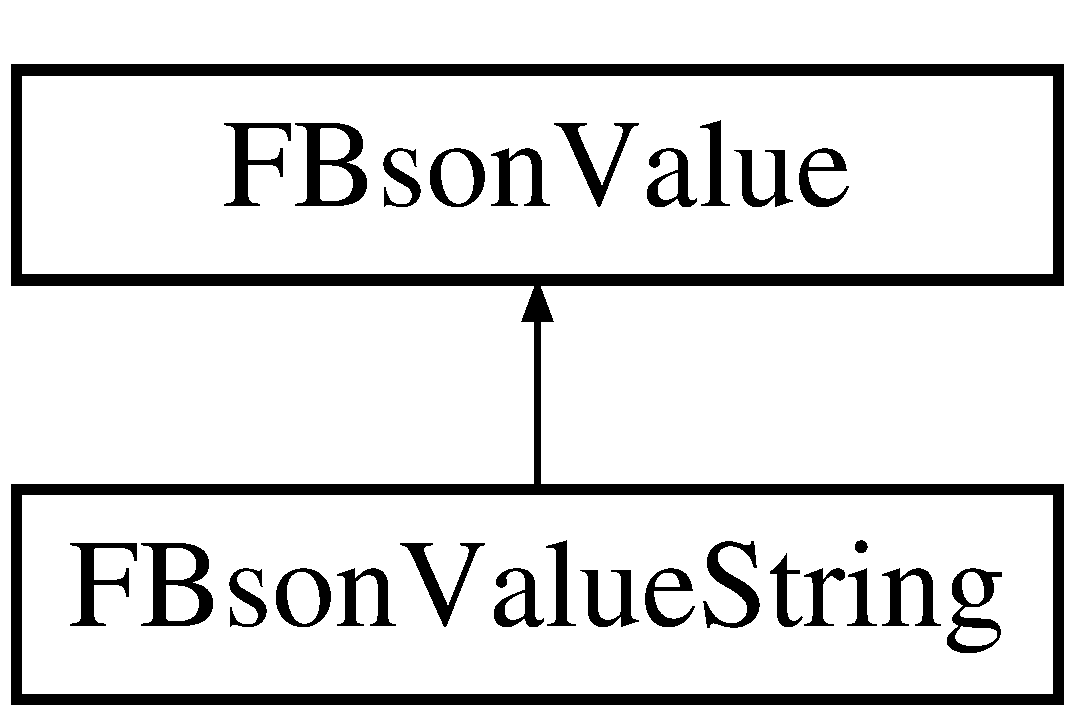
\includegraphics[height=2.000000cm]{class_f_bson_value_string}
\end{center}
\end{figure}
\subsection*{Public Member Functions}
\begin{DoxyCompactItemize}
\item 
\mbox{\Hypertarget{class_f_bson_value_string_aaed7b1cdf1a0194f63834a5f1cf9afea}\label{class_f_bson_value_string_aaed7b1cdf1a0194f63834a5f1cf9afea}} 
{\bfseries F\+Bson\+Value\+String} (const F\+String \&In\+String)
\item 
virtual bool \mbox{\hyperlink{class_f_bson_value_string_a531bcc8511d8de17418fd7fe6d0d797f}{Try\+Get\+String}} (F\+String \&Out\+String) const override
\item 
virtual bool \mbox{\hyperlink{class_f_bson_value_string_a7346681867daa27d7fa4a4e690ba55aa}{Try\+Get\+Number}} (double \&Out\+Double) const override
\item 
virtual bool \mbox{\hyperlink{class_f_bson_value_string_a81c2e67998032708c613773746c962bd}{Try\+Get\+Bool}} (bool \&Out\+Bool) const override
\end{DoxyCompactItemize}
\subsection*{Protected Member Functions}
\begin{DoxyCompactItemize}
\item 
\mbox{\Hypertarget{class_f_bson_value_string_a6978dea432d71e5f76ac9d226e830bc9}\label{class_f_bson_value_string_a6978dea432d71e5f76ac9d226e830bc9}} 
virtual F\+String {\bfseries Get\+Type} () const override
\end{DoxyCompactItemize}
\subsection*{Protected Attributes}
\begin{DoxyCompactItemize}
\item 
\mbox{\Hypertarget{class_f_bson_value_string_a4cb7ba55f5facf934531265b06bf9fb9}\label{class_f_bson_value_string_a4cb7ba55f5facf934531265b06bf9fb9}} 
F\+String {\bfseries Value}
\end{DoxyCompactItemize}
\subsection*{Additional Inherited Members}


\subsection{Detailed Description}
A Bson String Value. 

\subsection{Member Function Documentation}
\mbox{\Hypertarget{class_f_bson_value_string_a81c2e67998032708c613773746c962bd}\label{class_f_bson_value_string_a81c2e67998032708c613773746c962bd}} 
\index{F\+Bson\+Value\+String@{F\+Bson\+Value\+String}!Try\+Get\+Bool@{Try\+Get\+Bool}}
\index{Try\+Get\+Bool@{Try\+Get\+Bool}!F\+Bson\+Value\+String@{F\+Bson\+Value\+String}}
\subsubsection{\texorpdfstring{Try\+Get\+Bool()}{TryGetBool()}}
{\footnotesize\ttfamily virtual bool F\+Bson\+Value\+String\+::\+Try\+Get\+Bool (\begin{DoxyParamCaption}\item[{bool \&}]{Out\+Bool }\end{DoxyParamCaption}) const\hspace{0.3cm}{\ttfamily [inline]}, {\ttfamily [override]}, {\ttfamily [virtual]}}

Tries to convert this value to an boolean, returning false if not possible.


\begin{DoxyParams}{Parameters}
{\em Out\+Bool} & a reference to write the converted boolean into. \\
\hline
\end{DoxyParams}
\begin{DoxyReturn}{Returns}
false if value can\textquotesingle{}t be converted, true otherwise. 
\end{DoxyReturn}


Reimplemented from \mbox{\hyperlink{class_f_bson_value_a1c7d6b561d3cc8a7db99b850740c642e}{F\+Bson\+Value}}.

\mbox{\Hypertarget{class_f_bson_value_string_a7346681867daa27d7fa4a4e690ba55aa}\label{class_f_bson_value_string_a7346681867daa27d7fa4a4e690ba55aa}} 
\index{F\+Bson\+Value\+String@{F\+Bson\+Value\+String}!Try\+Get\+Number@{Try\+Get\+Number}}
\index{Try\+Get\+Number@{Try\+Get\+Number}!F\+Bson\+Value\+String@{F\+Bson\+Value\+String}}
\subsubsection{\texorpdfstring{Try\+Get\+Number()}{TryGetNumber()}}
{\footnotesize\ttfamily virtual bool F\+Bson\+Value\+String\+::\+Try\+Get\+Number (\begin{DoxyParamCaption}\item[{double \&}]{Out\+Double }\end{DoxyParamCaption}) const\hspace{0.3cm}{\ttfamily [inline]}, {\ttfamily [override]}, {\ttfamily [virtual]}}

Tries to convert this value to a double, returning false if not possible.


\begin{DoxyParams}{Parameters}
{\em Out\+Double} & a reference to write the converted number into. \\
\hline
\end{DoxyParams}
\begin{DoxyReturn}{Returns}
false if value can\textquotesingle{}t be converted, true otherwise. 
\end{DoxyReturn}


Reimplemented from \mbox{\hyperlink{class_f_bson_value_a519904f85122172ad9ca2f6b0b144f26}{F\+Bson\+Value}}.

\mbox{\Hypertarget{class_f_bson_value_string_a531bcc8511d8de17418fd7fe6d0d797f}\label{class_f_bson_value_string_a531bcc8511d8de17418fd7fe6d0d797f}} 
\index{F\+Bson\+Value\+String@{F\+Bson\+Value\+String}!Try\+Get\+String@{Try\+Get\+String}}
\index{Try\+Get\+String@{Try\+Get\+String}!F\+Bson\+Value\+String@{F\+Bson\+Value\+String}}
\subsubsection{\texorpdfstring{Try\+Get\+String()}{TryGetString()}}
{\footnotesize\ttfamily virtual bool F\+Bson\+Value\+String\+::\+Try\+Get\+String (\begin{DoxyParamCaption}\item[{F\+String \&}]{Out\+String }\end{DoxyParamCaption}) const\hspace{0.3cm}{\ttfamily [inline]}, {\ttfamily [override]}, {\ttfamily [virtual]}}

Tries to convert this value to an F\+String, returning false if not possible.


\begin{DoxyParams}{Parameters}
{\em Out\+String} & a reference to write the converted F\+String into. \\
\hline
\end{DoxyParams}
\begin{DoxyReturn}{Returns}
false if value can\textquotesingle{}t be converted, true otherwise. 
\end{DoxyReturn}


Reimplemented from \mbox{\hyperlink{class_f_bson_value_aa52379f3d911ed0d5c8ded6e83ceecc0}{F\+Bson\+Value}}.



The documentation for this class was generated from the following file\+:\begin{DoxyCompactItemize}
\item 
Bson\+Value.\+h\end{DoxyCompactItemize}

\hypertarget{class_f_u_e4_bson_module}{}\section{F\+U\+E4\+Bson\+Module Class Reference}
\label{class_f_u_e4_bson_module}\index{F\+U\+E4\+Bson\+Module@{F\+U\+E4\+Bson\+Module}}
Inheritance diagram for F\+U\+E4\+Bson\+Module\+:\begin{figure}[H]
\begin{center}
\leavevmode
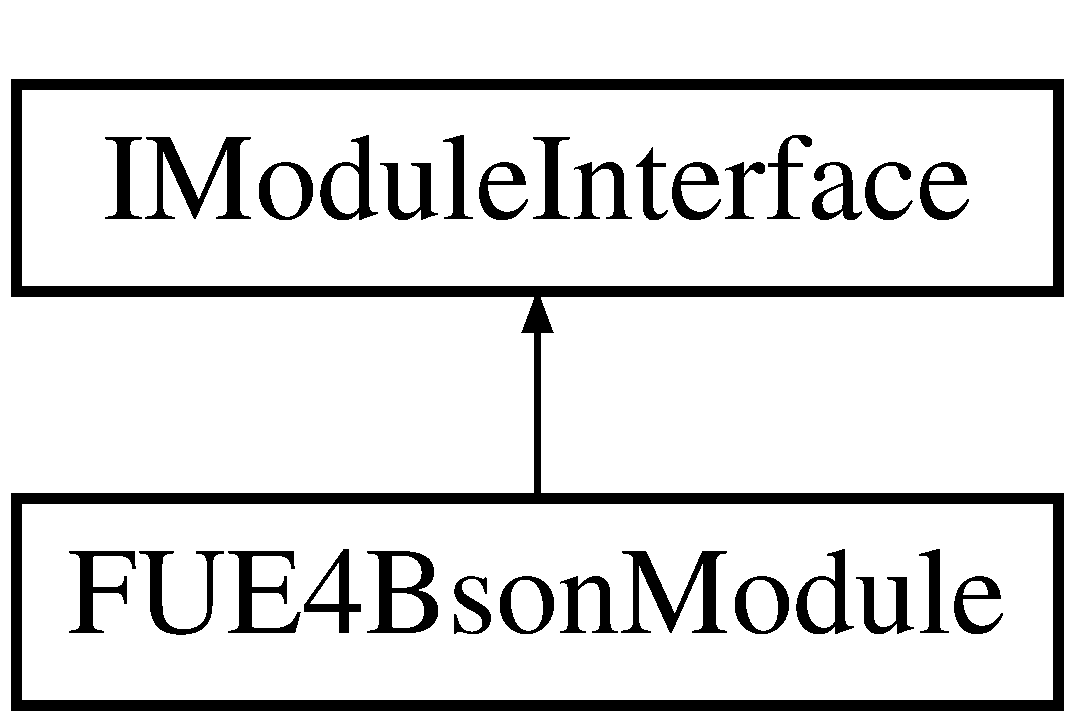
\includegraphics[height=2.000000cm]{class_f_u_e4_bson_module}
\end{center}
\end{figure}
\subsection*{Public Member Functions}
\begin{DoxyCompactItemize}
\item 
virtual void \mbox{\hyperlink{class_f_u_e4_bson_module_adcd0d99144d374de817306bb9e4229a5}{Startup\+Module}} () override
\item 
\mbox{\Hypertarget{class_f_u_e4_bson_module_a17c1e6aa5c7c8cd1d189873f0f830a63}\label{class_f_u_e4_bson_module_a17c1e6aa5c7c8cd1d189873f0f830a63}} 
virtual void {\bfseries Shutdown\+Module} () override
\end{DoxyCompactItemize}


\subsection{Member Function Documentation}
\mbox{\Hypertarget{class_f_u_e4_bson_module_adcd0d99144d374de817306bb9e4229a5}\label{class_f_u_e4_bson_module_adcd0d99144d374de817306bb9e4229a5}} 
\index{F\+U\+E4\+Bson\+Module@{F\+U\+E4\+Bson\+Module}!Startup\+Module@{Startup\+Module}}
\index{Startup\+Module@{Startup\+Module}!F\+U\+E4\+Bson\+Module@{F\+U\+E4\+Bson\+Module}}
\subsubsection{\texorpdfstring{Startup\+Module()}{StartupModule()}}
{\footnotesize\ttfamily virtual void F\+U\+E4\+Bson\+Module\+::\+Startup\+Module (\begin{DoxyParamCaption}{ }\end{DoxyParamCaption})\hspace{0.3cm}{\ttfamily [override]}, {\ttfamily [virtual]}}

I\+Module\+Interface implementation 

The documentation for this class was generated from the following file\+:\begin{DoxyCompactItemize}
\item 
U\+E4\+Bson.\+h\end{DoxyCompactItemize}

%--- End generated contents ---

% Index
\backmatter
\newpage
\phantomsection
\clearemptydoublepage
\addcontentsline{toc}{chapter}{Index}
\printindex

\end{document}
